%!TEX root = main.tex
\chapter{变分辨率正演与集合全波形反演方法} % (fold)
\label{cha:变分辨率正演与集合全波形反演方法}

地震正演是模拟地震发生时地震波传播的数值方法。正演是地震模拟的核心,也是反演的基础。正演过程在每个时刻不断更新地震波场,因此伴随着巨大的计算量,也是地震模拟最主要的计算开销。正演算法的性能直接影响着地震模拟和反演方法的效率,提升正演算法的性能具有重要的意义,也成了许多研究员和学者孜孜不倦的研究课题\cite{bednar2002limited,stork2013eliminating}。本章首先提出分时动态区域变分辨率正演方法,在正演过程中动态改变地震波场的更新范围和分辨率,有效地提升正演的性能。随后本章提出集合全波形反演方法,使用集合卡尔曼滤波中的集合协方差来近似完全反演中协方差算子,并引入震源编码算法克服局部收敛、提高运算效率。

% 地震波正演、逆时偏移算法、全波形反演算法等地球物理勘探算法的核心计算都是使用显式的有限差分算法更新地震波波场。
% 逆时偏移算法(reverse time migration,RTM)是人工地震成像中最常用,同时也是最耗时的算法之一。本章利用地震波能量在传播的过程中逐渐衰减的特性,提出逆时偏移衰减近似算法,在满足声波方程稳定性条件的情况下,逐渐提高网格的空间分辨率,并对不连续的网格进行插值,有效地降低了更新地震波波场的计算开销;并在太湖之光超算上并行优化。

\section{波动方程与正演算法} % (fold)

\subsection{声波方程} % (fold)
声波方程法是目前使用最普遍的正演算法。与射线法不同,声波方程法抛弃了高频假设,采用更准确的双向波动方程描述波场在介质中的传播。声波方程具有计算量适中、模型描述简单和准确性高等优点。

无阻尼、无强迫力介质中的声波方程的一阶形式为:
\begin{equation}
\left\{\begin{matrix}
\frac{\partial}{\partial t}P(\textbf{x},t) = -k(\textbf{x}) \triangledown \cdot v(\textbf{x}, t) \\
\frac{\partial}{\partial t}v(\textbf{x},t) = -\frac{1}{\rho(\textbf{x})} \triangledown \cdot P(\textbf{x}, t)
\end{matrix}\right.
\label{eq:waveeq}
\end{equation}
其中$\textbf{x}$表示空间位置,$t$表示时间,$P$和$v$是$(\textbf{x},t)$的函数,$k$为介质的体积模量,$\rho$为模型的密度。$P$为标量,表示$\textbf{x}$处质点在$t$时刻的压强。$v$为矢量,表示$\textbf{x}$处质点在$t$时刻的速度。公式\ref{eq:waveeq}可以消去$v$得到关于$P$的二阶形式:
\begin{equation}
  \frac{\partial ^2P(\textbf{x},t)}{\partial t^2} - k(\textbf{x})\triangledown \cdot (\frac{1}{\rho(\textbf{x})}P(\textbf{x},t))=0
  \label{eq:waveeq2}
\end{equation}
若$\rho$为常数,则方程\ref{eq:waveeq2}可以进一步简化为:
\begin{equation}
    \frac{\partial ^2P(\textbf{x},t)}{\partial t^2} - c(\textbf{x})^2\triangledown ^2 \cdot P(\textbf{x},t)=F(\textbf{x}, t)
  \label{eq:waveeq3}
\end{equation}
其中$c$为介质的声速,$F(\textbf{x}, t)$为额外引入的强迫压力项。一般情况下,方程\ref{eq:waveeq3}没有解析解,只能利用数值方法求解。

偏微分方程的定解条件还包括初始条件和边界条件。一般情况下初始条件为$P(\textbf{x},0)=0$,表示初始无振动。随着时间的推移,波源以$F(\textbf{x},t)=\delta(\textbf{x}-\textbf{x}_s)f(t)$的形式加入到介质空间$\textbf{x}_s$中,其中$\delta$为脉冲函数。脉冲函数有不同的形式,其中最常用的为Ricker子波。

边界条件为另外一个非常重要的定解条件,其中最简单的边界条件为自由反射边界,但并不符合实际地震模拟中的情景。地震数值模拟只对有限的区域空间进行模拟,而实际地震波却会无限制传播,因此常使用较复杂的吸收边界条件,如海绵吸收边界\cite{cerjan1985nonreflecting}、完美吸收边界\cite{berenger1994perfectly}。

% subsection 声波方程 (end)

\subsection{弹性波方程}

\subsubsection{控制方程}
弹性波方程是求解速度和应力张量耦合的偏微分方程,令
\begin{equation}
  v = (v_x, v_y, v_z)
  \label{eq:vvvv}
\end{equation}
表示波场中质点的速度向量,且令
\begin{equation}
  \sigma = \begin{pmatrix}
\sigma_{xx} & \sigma_{xy} & \sigma_{xz} \\
\sigma_{yx} & \sigma_{yy} & \sigma_{yz} \\
\sigma_{zx} & \sigma_{zy} & \sigma_{zz}
\end{pmatrix}
\end{equation}
为对称应力张量,则弹性动力学方程为
\begin{equation}
\begin{aligned}
\partial _t v &= \frac{1}{\rho}\triangledown \cdot \sigma  \\
\partial _{t}\sigma &= \lambda(\triangledown \cdot v)I + \mu(\triangledown \cdot v + \triangledown \cdot v^T)
\end{aligned}
  \label{eq:partialv}
\end{equation}
其中,$\lambda$和$\mu$是$lam\acute{e}$系数,$\rho$是介质密度。公式\ref{eq:partialv}可以将速度向量分解成三个标量方程,应力张量分解成六个标量方程。

地震波在地球内部传播过程中能量会逐渐衰减,这也必须体现在数值模拟中。本研究使用了品质因子$Q_s$和$Q_p$分别量化S波(横波)和P波(纵波)的滞弹性衰减。对于频率较高的情况,岩石和土壤中的非线性的响应以及盆地内浅层沉积岩的非线性行为会成为重要考虑因素。 为了适应这些非线性效应,本研究结合Drucker-Prager塑性 \citep {roten2016high},得到如下产量应力方程:
\begin{equation}
Y(\sigma)={\rm max}(0, c \cos \varphi - ( \sigma_{m} + P_{f} ) \sin\varphi)
\end{equation}
其中$c$为凝聚量(cohesion), $\varphi$为摩擦角度(friction angle), $P_{f}$为流体压力(fluid
pressure),$\sigma_{m}$为平均压力(mean stress)。产量函数也用以判断是否更新应力:
\begin{equation}
\sigma_{ij} = \sigma_{m}^{\rm trial} \delta_{ij} + r s_{ij}^{\rm{trial}}
\end{equation}
其中$r$ 是由产量应力$Y(\sigma)$计算所得,$s_{ij}$是应力偏导。

\subsubsection{交错网格有限差分方程}

公式\ref{eq:partialv}分解后的九个速度和应力标量方程可以用九个交错网格有限差分方程来近似。公式\ref{eq:staggedgrid}近似了交错网格有限差分方程的时间导数:
\begin{equation}
\begin{aligned}
  \partial_tv(t) &\approx \frac{v(t+\frac{\Delta t}{2})- v(t-\frac{\Delta t}{2})}{\Delta t} \\
\partial_{t} \sigma(t+\frac{\Delta t}{2}) &\approx \frac{\sigma(t+\Delta t) - \sigma(t)}{\Delta t}
\end{aligned}
  \label{eq:staggedgrid}
\end{equation}

速度和应力的空间导数可以用统一的方程描述。令$\Phi$表示速度或应力分量,$h$表示速度或应力网格中等距的空间分辨率,则网格点$(i,j,k)$的空间偏导$\partial_x \Phi$可以用如下有限差分方案近似:
\begin{equation}
  \partial_x \Phi(i,j,k) \approx D_x^4(\Phi)_{i,j,k} = \frac{c_1\left(\Phi_{i+\frac{1}{2},j,k} - \Phi_{i-\frac{1}{2},j,k}\right)+ c_2\left(\Phi_{i+\frac{3}{2},j,k} - \Phi_{i-\frac{3}{2},j,k}\right)}{h}
  \label{eq:staggedgridspatial}
\end{equation}
其中$c_1=9/8$,$c_2=-1/24$。公式\ref{eq:staggedgridspatial}可用以近似每个速度和应力分量中的空间导数。

\subsubsection{外部边界条件} % (fold)
\label{ssub:外部边界条件}
数值模拟网格在真实的地震波传播区域中截取的一部分。在数值模拟中,网格边界会对地震波造成反射现象,这与真实的地震波模拟不符。因此需要在数值模拟中添加吸收边界条件(absorb boundary condition, ABC),将地震波在边界处的反射现象降低至噪音的程度。最有效的吸收边界条件是完美匹配层(Perfectly Matched Layers,PML)吸收边界\cite{berenger1994perfectly,berenger1996three}。PML边界将波场分解成垂直和平行波场,并在垂直波场中添加吸收项。例如,将公式\ref{eq:partialv}中的$\triangledown$算子的$x$分量沿着垂直和平行方向分解成$\triangledown^{\perp x}$与$\triangledown^{\parallel x}$,速度和应力也可分解成$v^{\perp x}$、$v^{\parallel x}$、$\sigma^{\perp x}$和$\sigma^{\parallel x}$,则公式\ref{eq:partialv}可以分解成
\begin{equation}
  \begin{aligned}
    \partial _t v^{\perp x} &= \frac{1}{\rho}\triangledown ^{\perp x} \cdot \sigma  \\
    \partial _t v^{\parallel x} &= \frac{1}{\rho}\triangledown ^{\parallel x} \cdot \sigma  \\
\partial _{t}\sigma^{\perp x} &= \lambda(\triangledown ^{\perp x}\cdot v)I + \mu(\triangledown ^{\perp x} \cdot v + \triangledown ^{\perp x}\cdot v^T) \\
\partial _{t}\sigma^{\parallel x} &= \lambda(\triangledown ^{\parallel x}\cdot v)I + \mu(\triangledown ^{\parallel x} \cdot v + \triangledown ^{\parallel x}\cdot v^T)
  \end{aligned}
\end{equation}
边界的吸收项用$d(x)$来表示,将其添加到垂直波场的边界,可PML边界更新波场方程:
\begin{equation}
  \begin{aligned}
    \partial _t v^{\perp x} +d(x)v^{\perp x} &= \frac{1}{\rho}\triangledown ^{\perp x} \cdot \sigma  \\
    \partial _{t} + d(x)\sigma^{\perp x} &= \lambda(\triangledown ^{\perp x}\cdot v)I + \mu(\triangledown ^{\perp x} \cdot v + \triangledown ^{\perp x}\cdot v^T)
  \end{aligned}
\end{equation}

尽管PML边界吸收效果好,但在某些特定的情况(如边界处存在梯度很高的介质),PML边界会产生不稳定现象\cite{marcinkovich2002implementation}。因此,AWP-ODC实现了另一种吸收边界——海绵吸收边界\cite{cerjan1985nonreflecting}。虽然吸收效果不如PML边界,但缺拥有计算效率高和稳定等优点。

此外,为了模拟地球的自由表面,本文模型的顶部使用零应力自由表面条件\cite{gottschammer2001accuracy}。

\subsection{正演算法} % (fold)
有一系列数值方法能够模拟天然地震破裂和地震波传播过程,包括有限差分(finite difference)、有限元(finite element)、谱元(spectrum element)和有限体积(finite volume)方法。每种方法有各自最适合的应用场景,但从准确度、计算效率和编程实现难易程度综合考量,有限差分方法最适合用于地震波传播的数值模拟。

此处的正演算法是波动方程的数值解法,更狭义的指在规则网格上基于有限差分方法的波动方程显示时间解法。对于声波方程\ref{eq:waveeq3}的数值解法,本研究使用中心有限差分方法对二阶偏微分算子$\triangledown ^2$进行数值离散。例如,网格点$(ix, iy, iz)$在x方向的中心差分形式为:
\begin{equation}
  \frac{\partial ^2 P(ix, iy, iz)}{\partial x^2}=\frac{1}{dx^2}\sum_{k=-N}^N C_{|k|}P(ix+k, iy, iz)+O(dx^{2N+1})
\end{equation}
其中:
\begin{equation}
\left\{\begin{matrix}
\begin{aligned}
C_k &=\frac{(-1)^{k+1}\prod_{i=1,i\neq k}^N i^2}{k^2\prod_{i=i,i\neq k}^N |i^2-k^2|}\quad (k=1,2,\ldots,N) \\
C_0 &=-2\sum_{k=1}^N C_k  
\end{aligned}
\end{matrix}\right.
\end{equation}
该格式是$2N$阶精度差分。$\triangledown$空间的其他分量也可以同理进行差分离散化。中心差分格式展开后为星形的计算,空间中一点的二阶微分值由该点上下左右前后各$N$个点以及他本身的值共同计算决定(如图\ref{fig:stencilstruct}所示)。这种计算被称为$Stencil$运算,记为$\triangledown_s$。

\begin{figure}[ht]
  \centering
  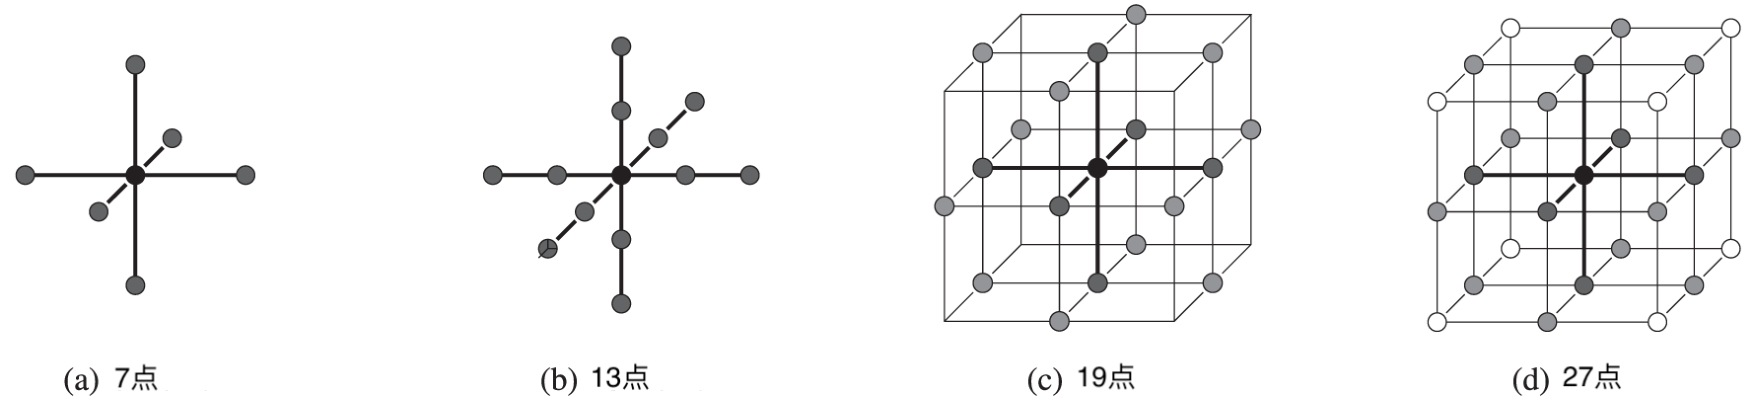
\includegraphics[width=0.9\columnwidth]{stencil7131927.pdf}
  \caption{不同stencil算子的空间结构\cite{zhang2013autogeneration}。(a)7点三维结构;(b)13点三维结构;(c)19点三维结构;(d)27点三维结构。}
  \label{fig:stencilstruct}
\end{figure}

在时间维度上,时间偏微分算子同样可用二阶形式的中心差分格式:
\begin{equation}
  \frac{\partial ^2 P(it)}{\partial t^2}=\frac{P(it+1)-2P(it)+P(it-1)}{dt^2}
\end{equation}
于是方程\ref{eq:waveeq3}在空间和时间经过二阶形式的中心差分离散化后可写成:
\begin{equation}
  P(it+1)=2P(it)-P(it-1)+\frac{c^2}{dt^2}\triangledown_s P(it)+F
  \label{eq:waveeq4}
\end{equation}
公式\ref{eq:waveeq4}为经典的基于二阶时间精度有限差分的波动方程数值解法。其中$P(it)$、$P(it+1)、$$P(it-1)$分别表示当前时刻、下一时刻和前一时刻的波场。

算法\ref{alg:acousticfdcode}是均匀介质三维声波正演伪代码,为了方便描述,使用的是基于2阶的有限差分算子\cite{fu2011eliminating}。但是2阶有限差分算子会带来严重的频散,实际生产和研究中,常常使用10阶或者12阶差分算子。

\begin{algorithm}[ht]
%\scriptsize
%\footnotesize
\small
\caption{均匀介质三维声波正演伪代码}\label{alg:acousticfdcode}
\begin{algorithmic}[1]
\State \textbf{for} ( it = 0; it < nt; it++ ) \{ \label{ln:fdntbegin}
\State \quad\quad \textbf{for} ( ix = 0; ix < nx; ix++ )
\State \quad\quad\quad\quad \textbf{for} ( iy = 0; iy < ny; iy++ ) \{
\State \quad\quad\quad\quad\quad\quad \textbf{for} ( iz = 0; iz < nz; iz++ )\{
\State \quad\quad\quad\quad\quad\quad\quad\quad  p(it,ix,iy,iz)=2*p(it-1,ix,iy,iz)-p(it-2,ix,iy,iz)+v(ix,iy,iz)*v(ix,iy,iz)*dt*dt*(
\State \quad\quad\quad\quad\quad\quad\quad\quad\quad\quad\quad\quad\quad\quad\quad                                    p(it-1,ix,iy,iz)*(2/dx/dx+2/dy/dy+2/dz/dz)+
\State \quad\quad\quad\quad\quad\quad\quad\quad\quad\quad\quad\quad\quad\quad\quad                                    (-p(it-1,ix,iy,ix-1)-p(it-1,ix,iy,ix+1))/dx/dx+
\State \quad\quad \quad\quad\quad\quad\quad\quad\quad\quad\quad\quad\quad\quad\quad                                    (-p(it-1,ix,iy-1,iz)-p(it-1,ix,iy+1,iz))/dy/dy+
\State \quad\quad\quad\quad\quad\quad\quad\quad\quad\quad\quad\quad\quad\quad\quad                                    (-p(it-1,iz-1,iy,iz)-p(it-1,iz+1,iy,iz))/dz/dz);
\State
\State \quad\quad\quad\quad\quad\quad\quad\quad \textbf{if} ( is\_boundary(ix, iy, iz) ) \textbf{//吸收边界处理} \label{ln:fdboundary}
\State \quad\quad\quad\quad\quad\quad\quad\quad\quad\quad\quad    apply\_absorb\_boundary\_condition(p);
\State \quad\quad\quad\quad\quad\quad                \} \label{ln:fdntend}
\State \quad\quad\quad\quad\quad\quad \textbf{if} (is\_record\_seismo) \textbf{//输出合成地震记录}
\State \quad\quad\quad\quad\quad\quad\quad\quad save\_seismo(p(it, ix, iy, :);
\State \quad\quad\quad\quad \}
\State
\State \quad\quad \textbf{if} ( is\_record\_wavefield ) \textbf{//输出波场快照}
\State \quad\quad\quad\quad output\_wavefield(p(it, :, :, :));
\State
\State \quad\quad \textbf{for} ( is = 0; is < ns; is++ ) \textbf{//在正传波场中添加震源信号}
\State \quad\quad\quad\quad p(it, src[is].x, src[is].y, src[is].z) += wavelet(is, it);
\State \}
\end{algorithmic}
\end{algorithm}

算法\ref{alg:acousticfdcode}仅描述了在一个速度模型样本,单个震源或者震源编码情况下的地震波正演。在传统的多震源正演中,不同震源之间是相互独立的,可以完全使用不同的节点分别对不同的震源进行地震波模拟,相互之间没有通信开销。因此,提升正演算子的性能只需要关注单个样本、单个震源下的地震波传播模拟即可。地震波正演过程中,核心计算是在$t=0$到$t=n-1$时刻不停往波场中注射震源激励信号、更新波场(第\ref{ln:fdntbegin}到\ref{ln:fdntend}行),并根据需要输出合成地震记录或者正传波场。

正演数值算法也需要在模拟区域的边界处添加吸收边界条件(第\ref{ln:fdboundary}到\ref{ln:fdntend}行),消除地震波在边界处的反射现象。

% subsection 正演算法 (end)

% section 波动方程与正演算法 (end)



% subsection 算法推导 (end)

% section 分时变分辨率正演方法 (end)

\section{分时动态区域变分辨率正演方法} % (fold)
\subsection{分时动态区域正演方法} % (fold)

\subsubsection{设计思路}
正演算法在每一个时间采样中更新地震波场的每一个格点。在地震波传播的初始阶段,波场中的每个格点被初始化为零,代表着该格点无信号。随后在震源处添加震源激励信号,通常为雷克子波函数,地震波的传播以震源为中心向四周扩散。图\ref{fig:地震波传播示例}描述了地震波在$t=0.1s$至$t=0.4s$处的波场快照。在地震波波前未到达模拟区域边界时,波前以外的区域仍处于初始状态,对应的数值为零。这为地震波正演提供了性能优化的空间。

\begin{figure}[ht]
  \centering
  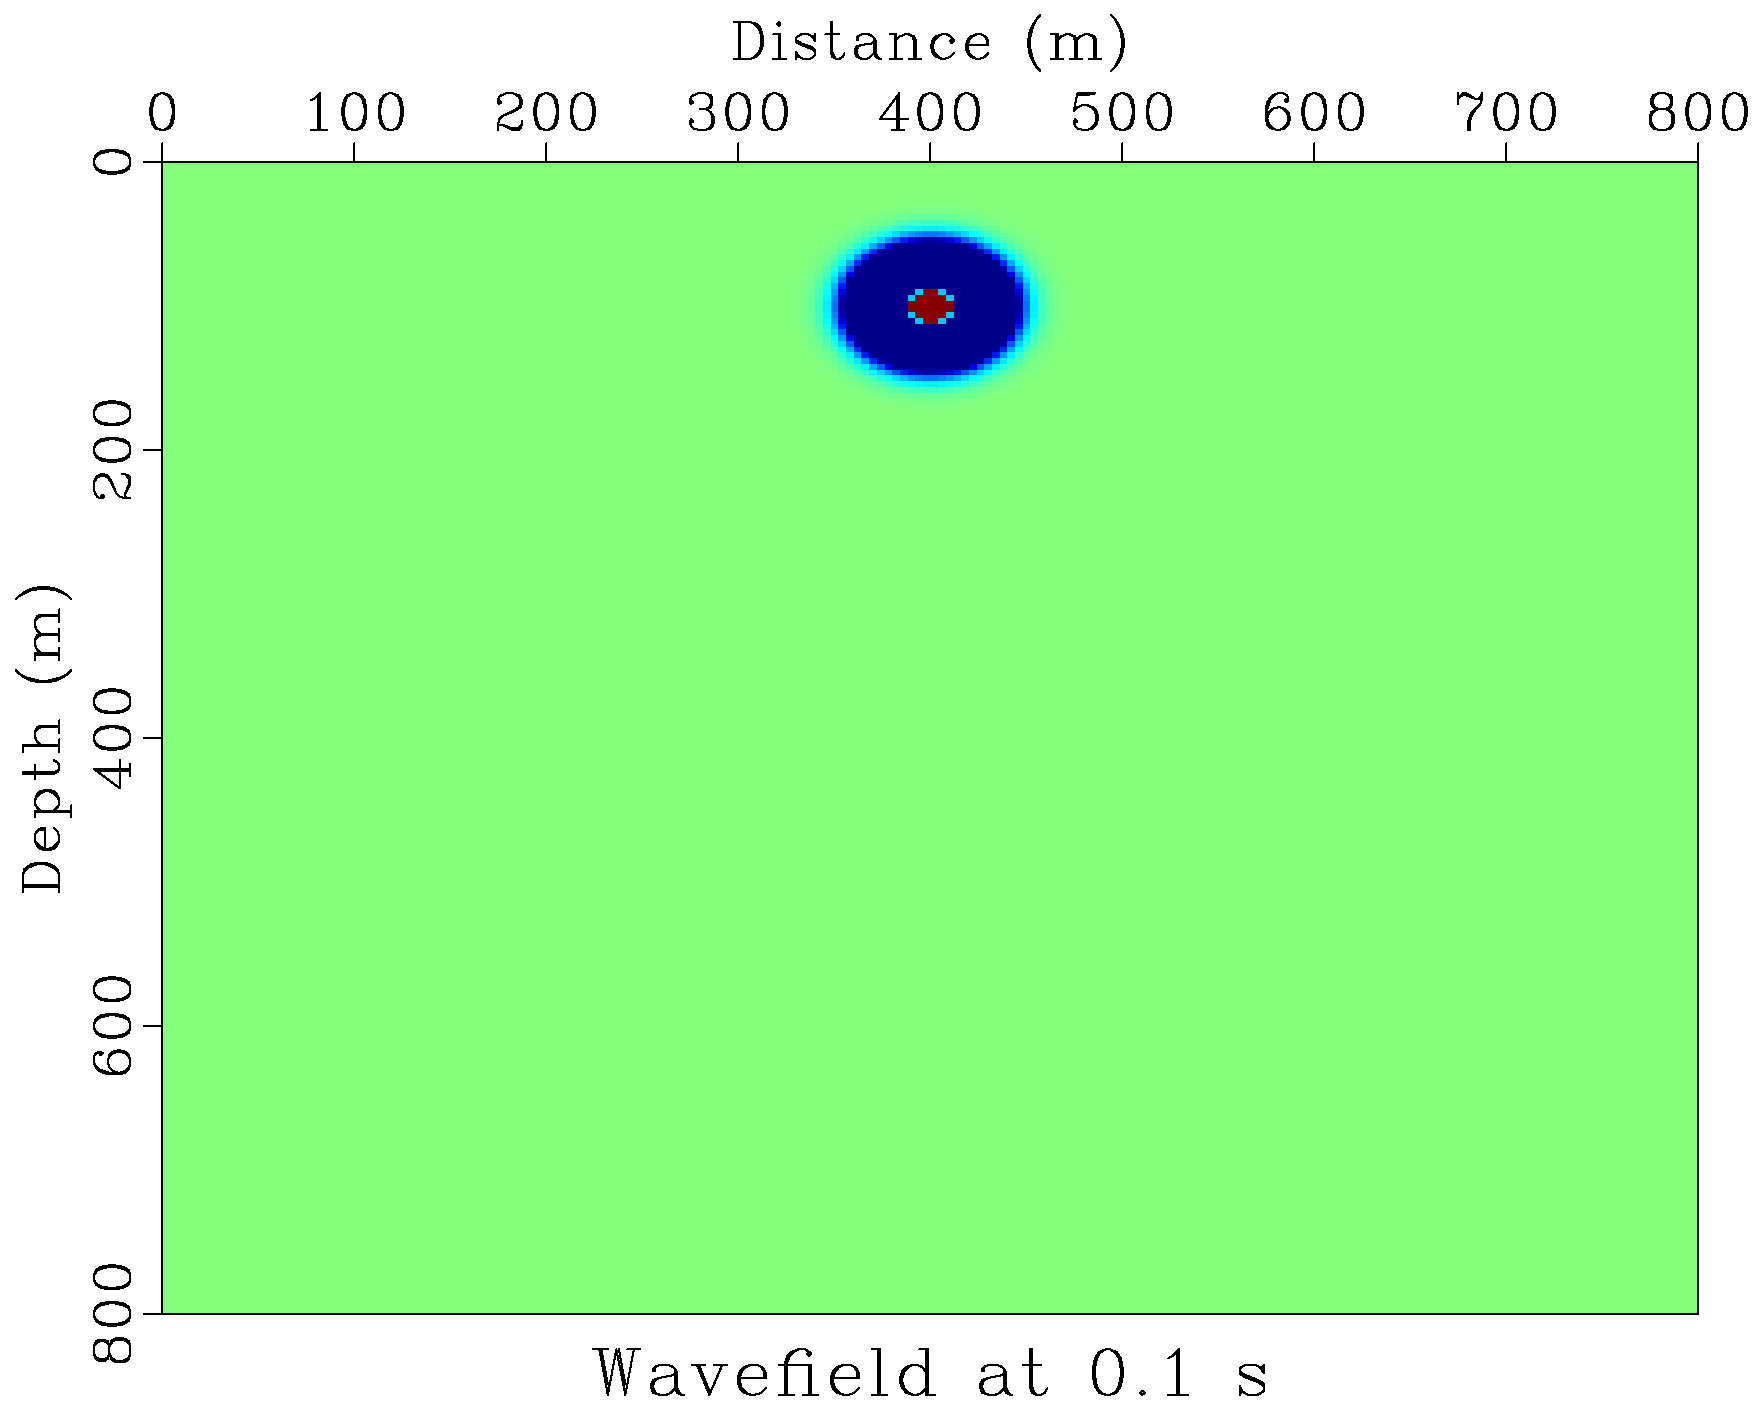
\includegraphics[width=0.24\textwidth]{wvl1.pdf}
  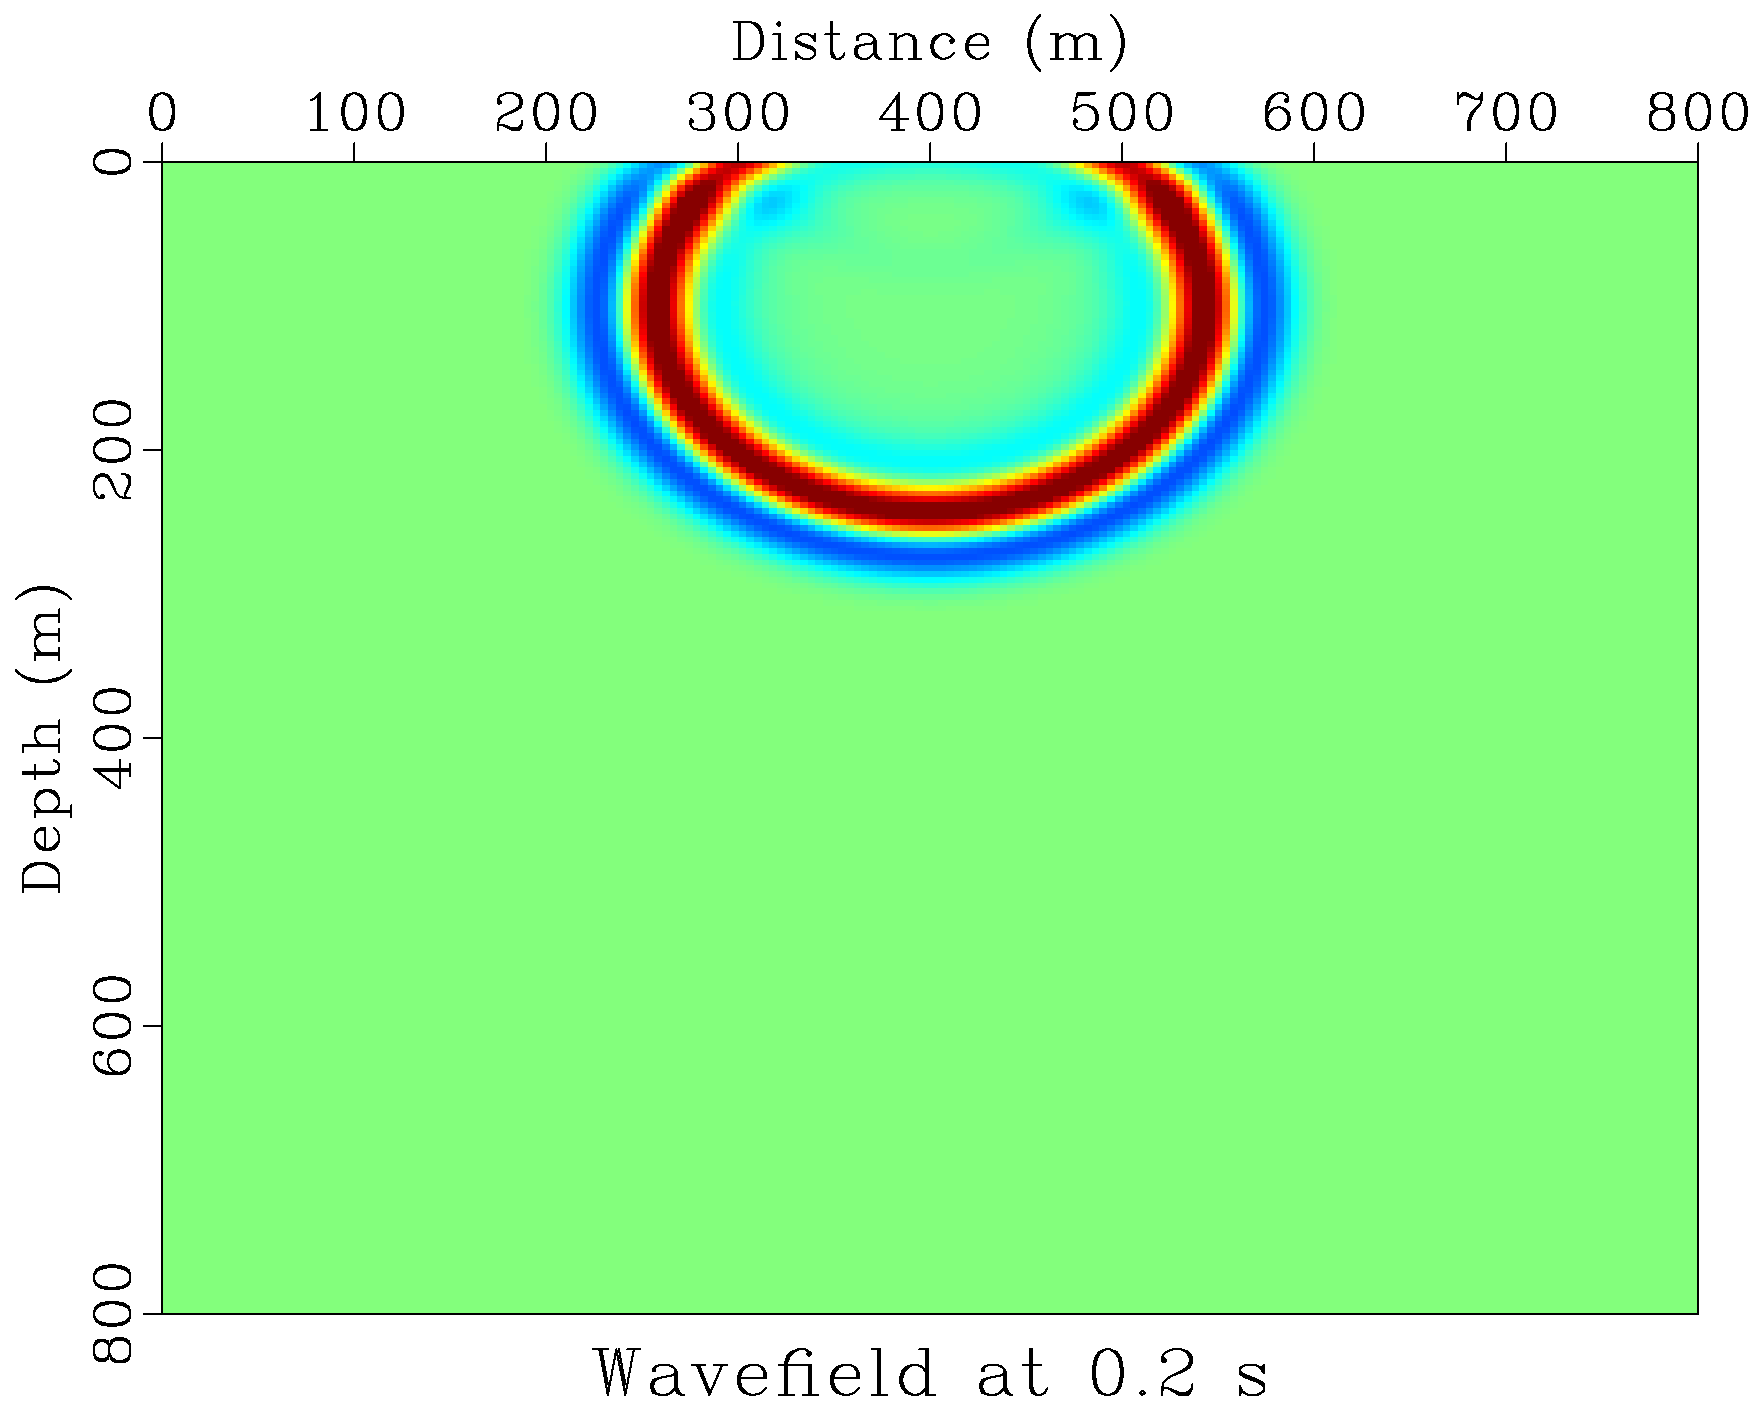
\includegraphics[width=0.24\textwidth]{wvl2.pdf}
  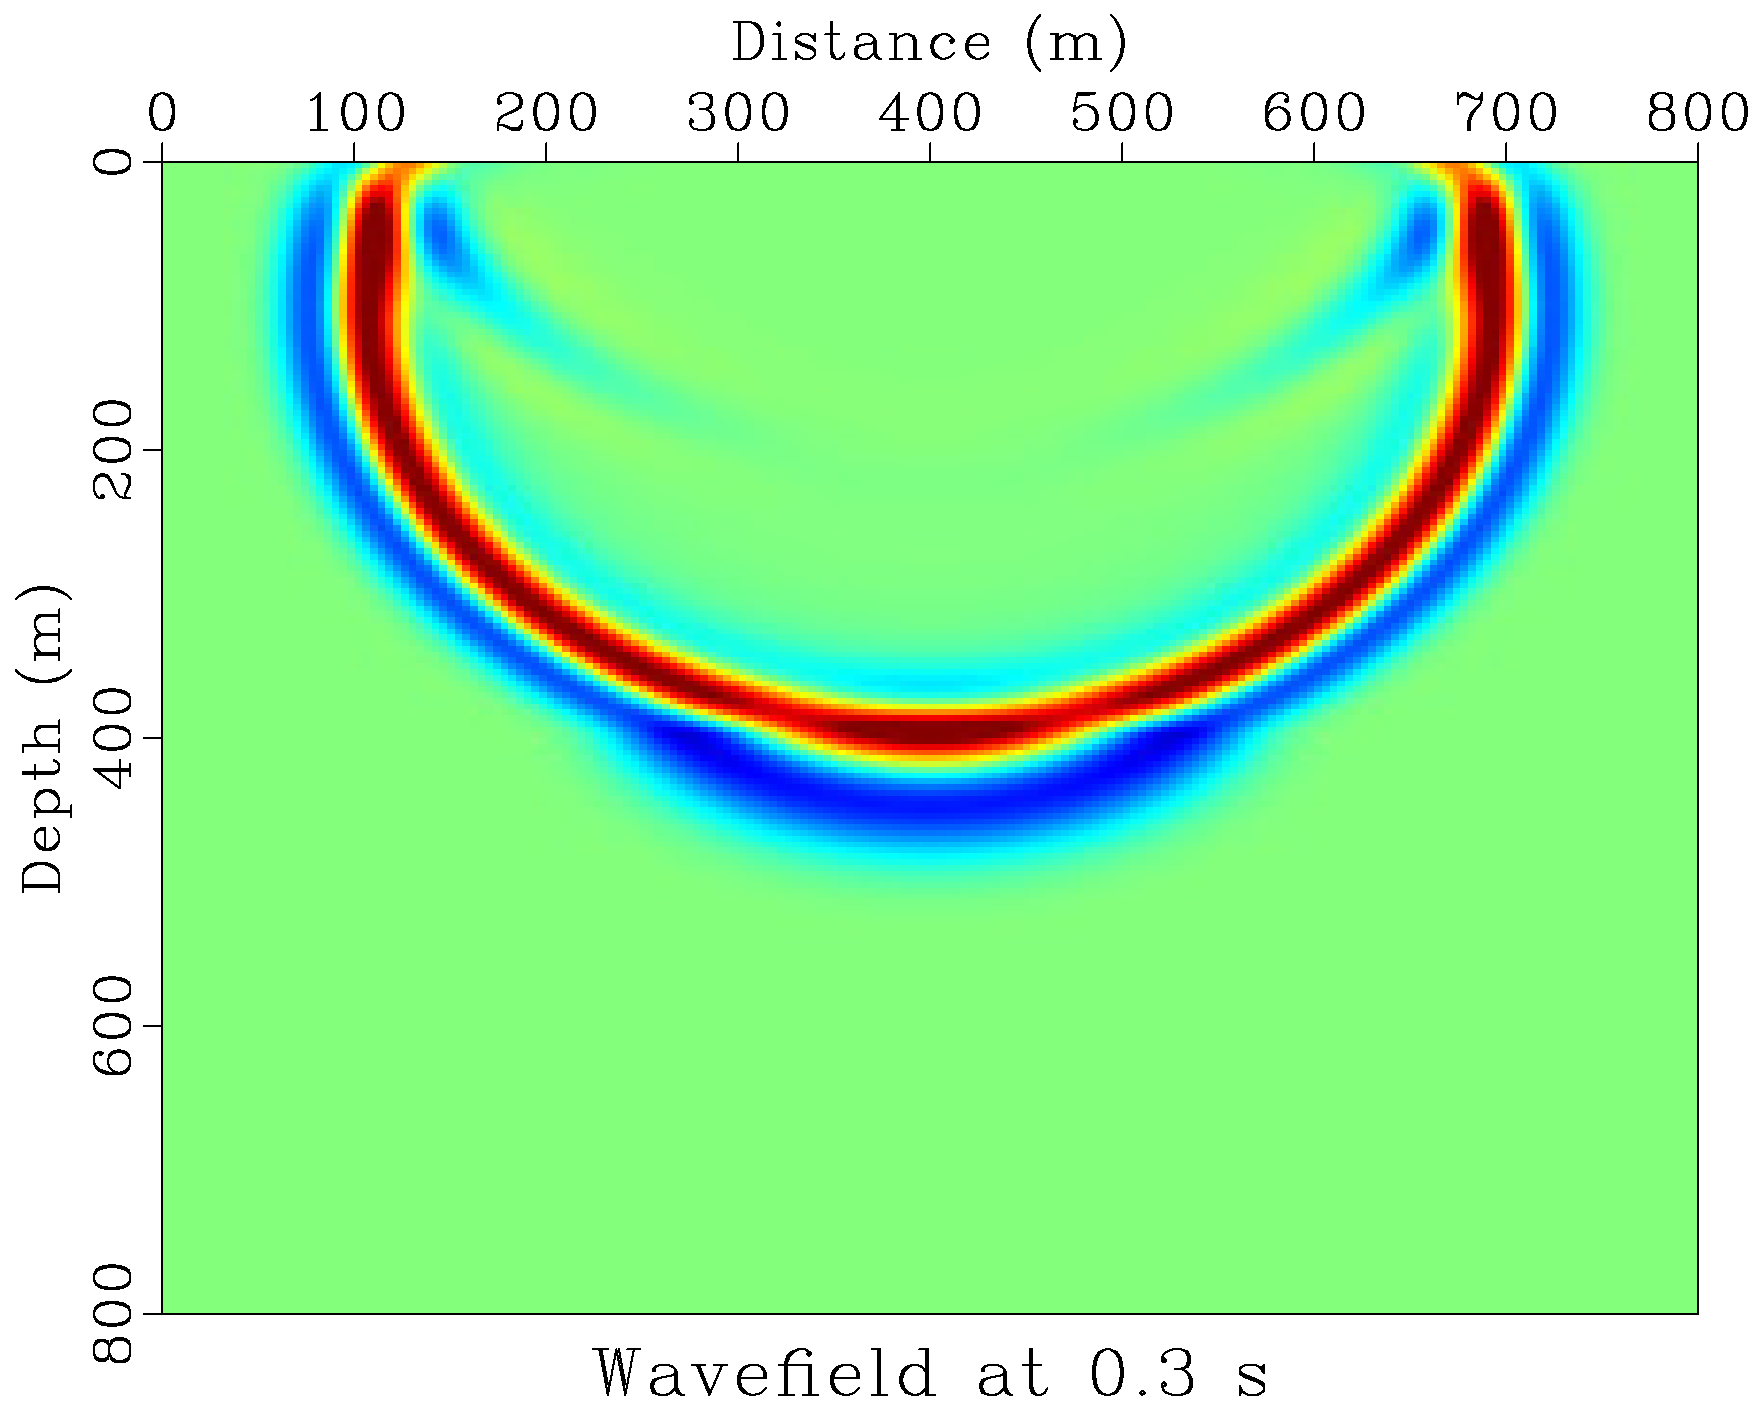
\includegraphics[width=0.24\textwidth]{wvl3.pdf}
  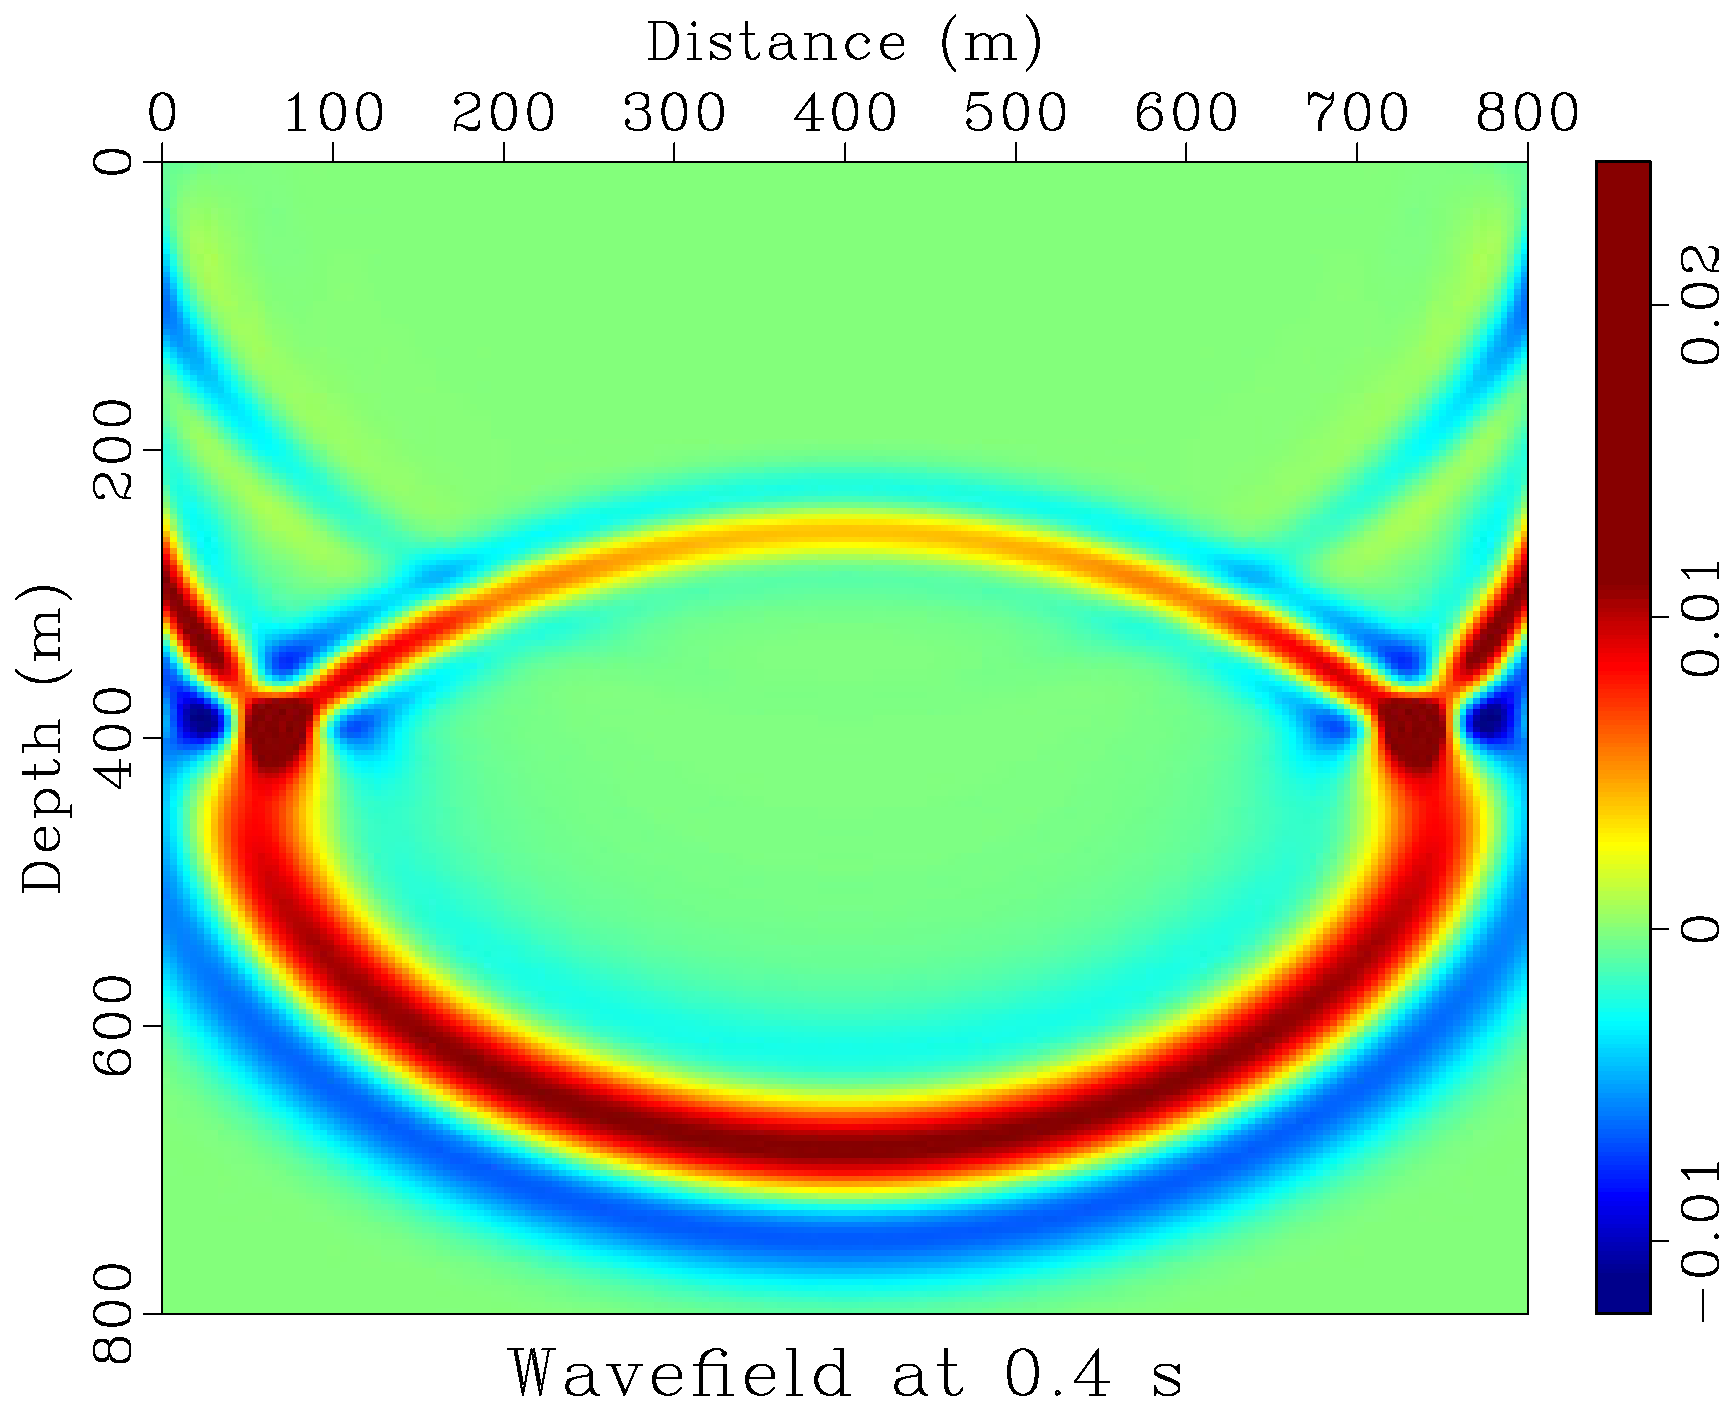
\includegraphics[width=0.24\textwidth]{wvl4.pdf}
  \caption{地震波在$t=0.1s$至$t=0.4s$处的波场快照。在地震波波前未到达模拟区域边界时,波前以外的区域仍处于初始状态,对应的数值为零。}
  \label{fig:地震波传播示例}
\end{figure}

对于地震波未到达的区域(数值为零),即便按照正演算法($Stencil$运算)更新完整的波场,该区域更新的数值仍旧为零,可认为这部分的计算为无效计算。在地震波正演初期,大部分的区域未受到波前的影响(如图\ref{fig:地震波传播示例}所示),而这部分区域的计算却占据了大量的计算周期。从图\ref{fig:地震波传播示例}还可以看到,传播时间越短,有效计算区域越小,无效计算区域越大。

本研究提出了分时动态区域正演方法,通过省去或者部分省去正演初期无效区域格点的更新,极大的降低地震波正演初期的计算开销,从而提升整体计算效率。

\subsubsection{算法描述}

分时动态区域算法由三个步骤组成:(1)将完整的正演时间分成若干小时间块(time block),(2)在每个小时间块中计算波前最大传播范围,(3)重新限定波场更新范围,在新的范围内执行常规正演计算。分时动态区域算法的伪代码如算法\ref{alg:varytime}所示。


\begin{algorithm}[ht]
%\scriptsize
%\footnotesize
\small
\caption{分时动态区域正演方法伪代码} \label{alg:varytime}
\begin{algorithmic}[1]
\State \textbf{// 将地震波完整传播时间分成nb块,每一块有不同的网格分辨率和地震波传播范围}
\State \textbf{for} (ib = 0; ib < nb; ib++) \{
\State \quad\quad cal\_max\_extend\_in\_timeblock(); \textbf{// 计算当前时间块波前能够传播的最大空间范围}
\State \quad\quad update\_range(); \textbf{// 更新计算范围}
\State \quad\quad
\State \quad\quad \textbf{for} (t = ib * nbt; t < ib * nbt + int; t++) \{ \textbf{// 每个时间块中执行常规正演运算}
\State \quad\quad\quad\quad modeling(); \textbf{// 按照新范围更新波场}
\State \quad\quad\quad\quad inject\_src(); \textbf{// 添加震源激励}
\State \quad\quad\quad\quad \textbf{if} (is\_imaging\_step(t))
\State \quad\quad\quad\quad\quad\quad save\_wavefield(); \textbf{// 存储波场}
\State \quad\quad \}
\State \}
\end{algorithmic}
\end{algorithm}

首先将完整的正演时间分成若干小时间块。在极端的情况下,正演过程中的每个时间步独立成为一个时间块,则总时间块数等于总时间步数。在这种情况下,无效计算区域最小,几乎每个时间步都在计算有效波场更新。然而这在节省无效计算开销的同时引入了额外的开销:在每个小时间块中计算波前最大传播范围。

在将完整的正演时间切分成若干小时间块后该如何确定该时间块内波前能够传播的最大范围?一般的情况下,只有完成该时间块内的正演操作时可以量化波前最大传播范围,这似乎与本步骤的需求相矛盾。地震波正演能够精确到每个格点的变化,而确定波前的最大传播范围无需跟踪每个格点的变化,只需关注波前即可。因此,本研究使用了基于射线的快速追赶法(fast march),在预处理阶段提前计算出每个时间块内波前能够达到的最远距离。快速追赶法的计算量与正演算法相比较小,可作为有效的预处理候选算法。值得注意的是正演过程通常包括多个震源,使用快速追赶法计算波前的最大传播范围时,应将所有震源的波前纳入计算范围。

确定了当前时间块地震波波前最大传播范围后,将新的传播范围内的空间作为当前时间块内需要更新的波场范围,然后执行常规的正演计算。


% section 分时动态区域正演方法 (end)

\subsection{分时变分辨率正演方法} % (fold)
\label{sec:分时变分辨率正演方法}

\subsubsection{设计思路}

稳定性条件限制了基于显式有限差分的正演算法中每个离散网格地震波能量的最大移动,因此稳定性条件是由模型中的最大速度$v_{max}$、最小空间采样$d_{min}$以及时间采样$dt$组成的函数(如公式\ref{eq:stability}所示)。
\begin{equation}
  v_{max} \frac{dt}{d_{min}} < 0.5
  \label{eq:stability}
\end{equation}

满足稳定性条件情况下,选择更大的空间采样可以获得更高的效率,但所得的分辨率更低;选择更小的空间采样可以提高结果分辨率,但需要更昂贵的计算开销。另一方面,频散是由模型中最小的速度$v_{min}$、最高的震源频率$f_{max}$以及最大的空间采样$d_{max}$组成的函数(如公式\ref{eq:dispersion}所示)。
\begin{equation}
  \frac{v_{min}}{f_{max}\cdot d_{max}} > 3
  \label{eq:dispersion}
\end{equation}

在给定的一次地震勘探实验中,$v_{min}$和$f_{max}$都是固定的,因此频散条件限制了网格的最大空间采样。当采用较小的空间采样以满足频散条件时,也必须采用较小的时间采样以满足稳定性条件。可以看到,降低频散假象是有限差分运算的最主要计算开销。地震波传播的计算开销与地震波能量频率呈四次方关系,频率的降低能极大降低计算开销。

地震波在地球内部传播时其能量会随着时间不断衰减,其中高频信息衰减最为明显。为了更精确描述真实地震波的传播现象,通常在波动方程中添加衰减因子Q表示能量的衰减,然而衰减因子的引入给地震波波场的更新带来额外的计算开销。

为了降低计算开销,本研究在\emph{Zhu, Tieyuan}和\emph{Harris, Jerry M}\cite{zhu2014modeling}的算法基础上提出了分时变分辨率正演方法,并将二维声波方程扩展到三维弹性波方程,有效的提高了地震波传播波场更新的效率。它一方面利用了地震波在地球内部传播时能量会不断衰减的特性,按照稳定性和频散条件的约束,增大了正演波场空间分辨率和时间采样;另一方面通过近似常数衰减因子来降低波动方程中添加衰减特性引入的大额计算开销。

\subsubsection{基于二维声波的常数衰减Q近似}
在实际观测中地球会吸收声波的能量。能量的衰减变化由波场频率和介质材料所决定。为了在可接受精度的前提下降低计算量,本研究采用常数衰减Q模型\cite{kjartansson1980attenuation}:
\begin{equation}
  Q = 2\pi(\frac{E}{\partial E})
\end{equation}
其中$\frac{E}{\partial E}$是每个周期中能量损失的部分。$Q$的值越大,每个周期中能量损失地越小。在常数Q的假设中,能量的衰减是一个通过介质的波长数量的函数,频率越高,能量衰减的越快,不受时间和空间分辨率的约束。有效的时间和空间分辨率保证地震波稳定传播,有效的空间分辨率保证地震波不出现频散等数值假象。

地震波波场的衰减在时间域的传播可以用分数拉普拉斯算子来完成\cite{zhu2014modeling}。给定震源函数$f(t)$以及波场$P(t)$,\emph{Zhu, Tieyuan}提出了公式\ref{eq:zhu}:
\begin{equation}
  f(t) = \left [ \eta L+\tau H\frac{d}{dt} -v^{-2} \frac{\partial ^2}{\partial t^2}\right ]P(t)
  \label{eq:zhu}
\end{equation}
其中,
\begin{equation}
  L = (-\triangledown ^2)^{\gamma + 1}
\end{equation}
\begin{equation}
  H = (-\triangledown ^2)^{\gamma + \frac{1}{2}}
\end{equation}
公式\ref{eq:zhu}中的衰减常数定义为
\begin{equation}
  \eta = -v^{2\gamma}w_0^{-2\gamma}\cos\pi\gamma
\end{equation}
\begin{equation}
  \tau = -v^{2\gamma-1}w_0^{-2\gamma}\sin\pi\gamma
\end{equation}
其中,
\begin{equation}
  \gamma = \frac{1}{\tan^{-1}\frac{1}{Q}}
\end{equation}
公式\ref{eq:zhu}中的第一项$\eta L$处理波场衰减中的频散效应,第二项$\tau H\frac{d}{dt}$处理波场衰减。如果使用常数衰减Q近似,即使用$\triangledown ^2$近似$H$,则公式\ref{eq:zhu}可以进一步演化为
\begin{equation}
  f(t) = \left [ \triangledown ^2 +\tau \triangledown ^2\frac{d}{dt} -v^{-2} \frac{\partial ^2}{\partial t^2}\right ]P(t)
  \label{eq:bob2d}
\end{equation}
公式\ref{eq:bob2d}为常数衰减Q近似二维声波波场传播公式。

\subsubsection{基于三维弹性波的常数衰减Q近似}

在线性化弹性理论和应力刚度张量公式的假设下\cite{landau1986theory},公式\ref{eq:prop3d}描述使用数值模拟实现三维弹性波在横向各向同性介质中的传播。
\begin{equation}
  \epsilon_{kl} = \frac{1}{2}\left[ \partial_k u_l + \partial_l u_k\right], \quad\quad k,l = 1,2,3
  \label{eq:prop3d}
\end{equation}
其中$\epsilon_{kl}$是线性拉力张量元素,$\partial_k$是第$k$个方向上的空间偏导,$u_l$是弹性波波场第$l$个方向的位移。本文中使用的笛卡尔空间坐标系中的$x, y, z$坐标轴分别使用下标$i=1, 2, 3$表示。

线性拉力张量$\epsilon_{kl}$与高斯应力张量$\sigma_{ij}$的关系如通过公式\ref{eq:strainstress}所示。它通过四阶刚度张量$c_{ijkl}$描述了弹性介质的属性。
\begin{equation}
  \sigma_{ij} = c_{ijkl}\cdot \epsilon_{kl}
  \label{eq:strainstress}
\end{equation}

根据牛顿第二定律,上述方程可以组合成运动学方程,描述波通过各向异性弹性介质的传播:
\begin{equation}
  \rho \partial_{tt}^2u_i=\partial_j \sigma_{ij}+F_i
  \label{eq:partialtt}
\end{equation}
其中$F_i$是每个三维体中的应力源,$\rho$是介质密度,$\partial_{tt}^2$是时间二阶偏导。

在此基础上,将公式\ref{eq:zhu}从二维粘弹性扩展到三维粘弹性场景。扩展过程中,分数阶Laplacian偏微分算子为弹性建模带来了额外的计算成本,这背离了本研究提升波场传播效率的初衷,因此本研究使用传统的整数阶Laplacian算子对其进行近似,这不仅显着降低了计算复杂性,而且在$Q$值不是非常低时仍保持了精度\cite{shen2015image}。因此,公式\ref{eq:appro3d}为扩展后的常数衰减Q近似三维弹性波波场传播公式。
\begin{equation}
\begin{aligned}
\begin{bmatrix} \sigma_{11}\\ \sigma_{22}\\ \sigma_{33} \end{bmatrix} &= \begin{bmatrix} \frac{\partial \tau_p^{(1)}}{\partial t} + c_{11} & \frac{\partial \tau_p^{(1)}}{\partial t} - 2\frac{\partial \tau_s^{(1)}}{\partial t} +c_{12}& \frac{\partial \tau_p^{(1)}}{\partial t} - 2\frac{\partial \tau_s^{(1)}}{\partial t} +c_{13} \\ \frac{\partial \tau_p^{(2)}}{\partial t} - 2\frac{\partial \tau_s^{(2)}}{\partial t} +c_{12}& \frac{\partial \tau_p^{(2)}}{\partial t} + c_{22} & \frac{\partial \tau_p^{(2)}}{\partial t} - 2\frac{\partial \tau_s^{(2)}}{\partial t} +c_{23}\\ \frac{\partial \tau_p^{(3)}}{\partial t} - 2\frac{\partial \tau_s^{(3)}}{\partial t} +c_{13} & \frac{\partial \tau_p^{(3)}}{\partial t} - 2\frac{\partial \tau_s^{(3)}}{\partial t} +c_{23} & \frac{\partial \tau_p^{(3)}}{\partial t} + c_{33} \end{bmatrix} \begin{bmatrix} \epsilon_{11}\\ \epsilon_{22}\\ \epsilon_{33} \end{bmatrix} \\
\sigma_{12} &= \left ( 2\frac{\partial}{\partial t} \left( \frac{c_{11}-c_{12}}{2}c_s^{(2\gamma_s-1)}\sin(\pi\gamma_s) \right) + c_{66} \right )\times \epsilon_{12}\\
\sigma_{13} &= \left ( 2\frac{\partial}{\partial t} \left( \frac{c_{33}-c_{13}}{2}c_s^{(2\gamma_s-1)}\sin(\pi\gamma_s) \right) + c_{55} \right )\times \epsilon_{13} \\
\sigma_{23} &= \left ( 2\frac{\partial}{\partial t} \left( \frac{c_{22}-c_{23}}{2}c_s^{(2\gamma_s-1)}\sin(\pi\gamma_s) \right) + c_{44} \right )\times \epsilon_{23}
\end{aligned}
\label{eq:appro3d}
\end{equation}
其中,$\sigma_{i,j}$是应力(stress)张量,$\epsilon_{i,j}$是拉力(strain)张量,$c_{ij}$四阶刚度(stiffness)张量。公式\ref{eq:taups}给出了$\tau_p^{(1)}$和$\tau_s^{(1)}$的计算:
\begin{equation}
\begin{aligned}
  \tau_p^{(1)} &= c_{11}C_p^{2\gamma_p - 1}\sin(\pi \gamma_p) \\
  ~
  \tau_s^{(1)} &= \frac{c_{11} - c_{13}}{2}C_s^{2\gamma_s - 1}\sin(\pi \gamma_s)
\end{aligned}
\label{eq:taups}
\end{equation}
且,
\begin{equation}
  \gamma_{p,s}=\frac{1}{\pi}\tan^{-1}(\frac{1}{Q_{p,s}})
\end{equation}
其中$C_p$和$C_s$分别为模型的横波(S波)和纵波(P波)速度,$Q_{p,s}$分别是纵波横波所对应的常量衰减因子。注意,本文只给出了$\tau_p^{(1)}$和$\tau_s^{(1)}$的计算公式,$\tau_p^{(2)}$、$\tau_p^{(3)}$、$\tau_s^{(2)}$以及$\tau_s^{(3)}$可以用类似的方法推导得出。

上述推导的常数衰减Q近似三维弹性波波场传播方法能够提升计算效率有以下主要原因:
\begin{itemize}
  \item 使用传统的Laplacian算子近似分数阶的Laplacian算子,降低了计算复杂度;
  \item 推导的过程中,忽略了公式\ref{eq:zhu}中的频散项,但几乎不会对计算精度造成影响\cite{shen2015image};
  \item 保留了原来的三维弹性波方程正演的计算流程,仅在计算张力和应力张量时添加了额外的计算项。
\end{itemize}

数值试验模拟需要对上述公式进行离散化。本文定义计算网格的大小为$N_x \times N_y \times N_z$,地震波传播的时间步为$N_t$,地震波场中的任意时刻任意点可以表述为$(x,y,z|t)=(p\Delta x,q\Delta y, r\Delta z| n\Delta t)$,其中计数器$p,q,r,n$的范围为$p=[1,N_x], q=[1,N_y], r=[1,N_z], n=[1,N_t]$。则连续地震波波场位移中的任意一点通过离散网格表示为:
\begin{equation}
  u_i|_{x,y,z|t} \approx u_i^{p,q,r|n}
\end{equation}

一阶偏导$\partial_j$可通过八阶的中心差分算子$D_x[\cdot]$来近似\cite{trefethen1996finite}:
\begin{equation}
  \partial_x u_j \approx D_x[u_j^{p,q,r|n}] = \frac{1}{\Delta x}\sum_{\alpha=1}^4W_\alpha\left(u_j^{p+\alpha,q,r|n} - u_j^{p-\alpha,q,r|n}\right)
  \label{eq:partialx}
\end{equation}
其中$W_\alpha$为二项式的权重之一,所有的权重为$W=\left[ \frac{+4}{5}, \frac{-1}{5}, \frac{+4}{105}, \frac{-1}{280}\right]$。对于$y$轴和$z$轴的偏导可以类似公式\ref{eq:partialx}通过空间差分算子$D_y[\cdot]$和$D_z[\cdot]$获得,并将三个差分算子代入公式\ref{eq:partialtt}中,然后使用标准的时间二阶精度近似可得
\begin{equation}
  \partial_{tt}^2u_j \approx D_{tt}u_j^{p,q,r|n}=\frac{1}{\Delta t^2}\left[ u_j^{p,q,r|n+1} - 2u_j^{p,q,r|n} + u_j^{p,q,r|n-1} \right]
\end{equation}

将上述差分算子代入公式\ref{eq:partialtt}中即可通过有限差分算子进行三维弹性波正演的数值实验模拟。

\subsection{分时动态区域变分辨率正演方法}
分时动态区域正演方法和分时变分辨率正演方法可以在同一个时间块进行有机结合形成分时动态区域变分辨率正演方法。在同一个时间块内同时确定新的正演范围和正演时空分辨率。算法\ref{alg:qforward}是分时动态区域变分辨率正演方法伪代码。

\begin{algorithm}[ht]
%\scriptsize
%\footnotesize
\small
\caption{基于常数衰减近似的地震波正演伪代码} \label{alg:qforward}
\begin{algorithmic}[1]
\State \textbf{// 将地震波完整传播时间分成nb块,每一块有不同的网格分辨率和地震波传播范围}
\State \textbf{for} (ib = 0; ib < nb; ib++) \{ \label{ln:qfwdnb}
\State \quad\quad cal\_max\_freq\_for\_timeblock(); \textbf{// 计算当前时间块地震波剩余最大频率} \label{ln:calfreq}
\State \quad\quad cal\_max\_extend\_in\_timeblock(); \textbf{// 计算当前时间块地震波能够传播的最大空间范围} \label{ln:calextend}
\State \quad\quad cal\_sampling(); \textbf{// 根据稳定性和频散条件计算当前时间块新的网格空间和时间分辨率} \label{ln:calsampling}
\State \quad\quad resample(); \textbf{// 将旧网格按照新空间分辨率插值得到新网格} \label{ln:resample}
\State \quad\quad
\State \quad\quad \textbf{for} (t = ib * nbt; t < ib * nbt + int; t++) \{ \textbf{// 每个时间块中执行常规正演运算} \label{ln:tbbegin}
\State \quad\quad\quad\quad fwd\_prop\_appr\_q(); \textbf{// Q近似波场更新}
\State \quad\quad\quad\quad inject\_src(); \textbf{// 添加震源激励}
\State \quad\quad\quad\quad \textbf{if} (is\_imaging\_step(t))
\State \quad\quad\quad\quad\quad\quad save\_wavefield(); \textbf{// 为RTM成像存储波场} \label{ln:savewavefield}
\State \quad\quad \} \label{ln:tbend}
\State \} \label{ln:qfwdnbend}
\end{algorithmic}
\end{algorithm}

常规的地震波正演算法采用统一的网格分辨率来计算$t=0\ldots nt$地震波波场的更新。分时动态区域变分辨率正演方法在常规正演的基础上添加了以下流程:
\begin{itemize}
  \item 将完整的地震波传播时间分成$nb$块(time block),每个时间块都对应着不同的波场网格分辨率和地震波传播范围(第\ref{ln:qfwdnb}到\ref{ln:qfwdnbend}行)。
  \item 在每个时间块的内部,首先计算地震波从震源传播到当前时间块的起始时间剩余的最大频率(第\ref{ln:calfreq}行)。随着地震波传播的时间递增,当前时间块起始时间的最大频率会不断缩小,这是调节空间分辨率的前提。
  \item 使用快速追踪算法\cite{um1987fast}计算当前时间块地震波能够传播的最大空间范围(第\ref{ln:calextend}行)。传统的正演算法并不考虑地震波波前的位置,在设置好边界条件之后对完整的地震波传播区域进行更新。但在地震波传播的早期,有效的地震波仅在以震源为中心的三维空间中传播,其余位置都处于初始状态,这部分波场更新后的与更新前相同,因此更新这部分的计算是冗余。在地震波传播前,根据震源的位置通过射线追踪算法计算出每个时间块结束时地震波能到抵达的最大空间范围,然后重新限定网格的计算区域,能有效地降低计算量。时间块划分地越精细、传播时间越早,节约的计算时间则越多。
  \item 根据稳定性和频散条件计算当前时间块新的网格空间分辨率(第\ref{ln:calsampling}行)。基于常数衰减近似地震波正演算法计算新的网格空间分辨率,是提升性能的关键。相同物理传播区域内计算开销与空间分辨率成呈正相关。对于三维模拟,计算开销与空间分辨率呈三次方关系,因此降低空间分辨率能极大地节约计算成本。由于稳定性和频散约束条件的限制,空间分辨率无法任意取值。本算法通过模拟实际地震波能量衰减的现象,在数值模拟中不断降低波场最高频率,并根据稳定性和频散约束条件,降低空间和时间分辨率来提高计算效率。
  \item 将旧网格按照新空间分辨率插值得到新网格(第\ref{ln:resample}行)。这是该算法引入的主要额外计算开销。每一个时间块中的空间分辨率都基本不同,划分的时间块越多会导致插值的次数越多,额外引入的插值计算开销也就越大。另一方面,在不考虑插值开销的情况下,划分的时间块越多,本算法能获得的性能提升越大。因此需要在本算法获得的性能提升与引入的额外开销之间进行平衡,找到较优的划分方法。
\end{itemize}

根据新计算的空间分辨率对网格插值之后,采用与算法\ref{alg:acousticfdcode}相同的方式进行地震波正演(第\ref{ln:tbbegin}到\ref{ln:tbend}行)。在存储波场的时间步中(第\ref{ln:savewavefield}行)有两种方式。(1)直接将插值后的波场以及相应的参数配置(如当前网格分辨率,网格范围等等)输出,后续需要用到相应数据时(如逆时偏移算法或者可视化)再重新进行插值;(2)对所有网格按照原始网格的大小进行插值,统一得到相同大小的网格,然后输出。本文建议并采用方法(1),理由包括:
\begin{itemize}
  \item 当前时间窗口中的网格空间采样较高,输出到硬盘的文件较小,降低了运行时IO的开销。
  \item 将程序划分为预处理、核心计算和后处理,有助于提高各类资源利用率,也更利于流水化。
\end{itemize}

\subsection{算法分析} % (fold)

本研究进行了数值实验模拟验证了分时动态区域变分辨率正演方法的正确性和性能提升。正演的背景速度模型是大小为$700\times700\times700$的三维网格,其中空间分辨率为$dx=dy=dz=10m$,速度模型中横波和纵波速度分别为$vp=2000m/s, vs=1154.7m/s$,接收器平铺在网格的顶部平面的每一个点,范围为$rnx=rny=700, rdx=rdy=10m$;震源采用初始频率为$10Hz$的雷克子波;地震波正演的总时长为$8s$,时间步长为$2ms$,总时间步为$nt=4000$。

图\ref{fig:无衰减的地震波正演波场在$t=0.8s$的波场快照。}是使用上述配置运行的无衰减的地震波正演波场在$t=0.8s$的波场快照(只截取了三维速度模型中$z$方向分量的$x-z$平面,其他分量或其他平面也可得类似的结果),这作为对比基准。图\ref{fig:常数衰减近似的地震波正演波场在$t=0.8s$的波场快照。}是使用与对比基准相同配置的同时添加了$Q_s=Q_p=20$的常数衰减因子的正演波场快照结果。从整体上看,这两个波场快照几乎相同,没有出现频散以及其他假象,这说明常数衰减近似算法能够保证正演结果的正确性。

\begin{figure}[ht]
    \centering
    \begin{subfigure}[b]{0.5\textwidth}
        \centering
        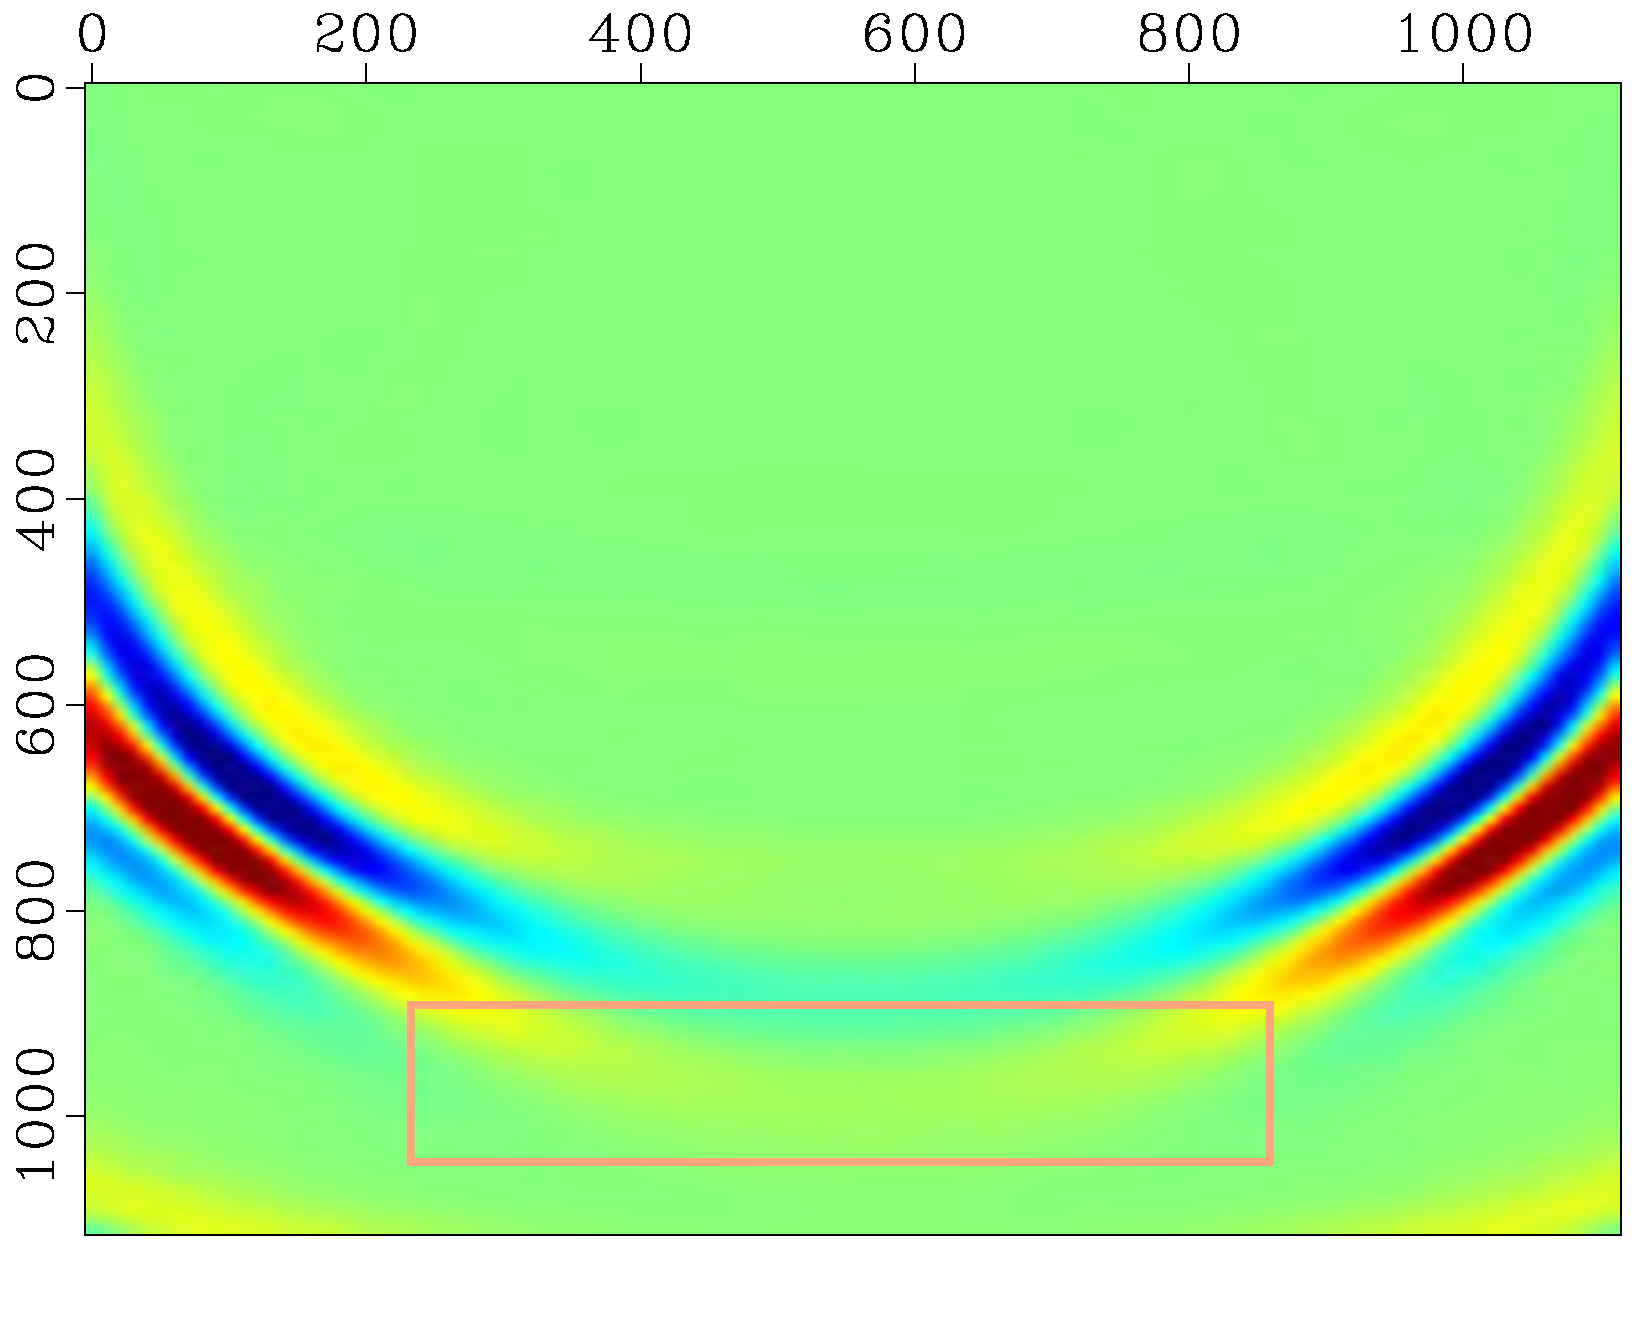
\includegraphics[height=2.2in]{std.pdf}
        \caption{无衰减的地震波正演波场在$t=0.8s$的波场快照。}
        \label{fig:无衰减的地震波正演波场在$t=0.8s$的波场快照。}
    \end{subfigure}%
    ~
    \begin{subfigure}[b]{0.5\textwidth}
        \centering
        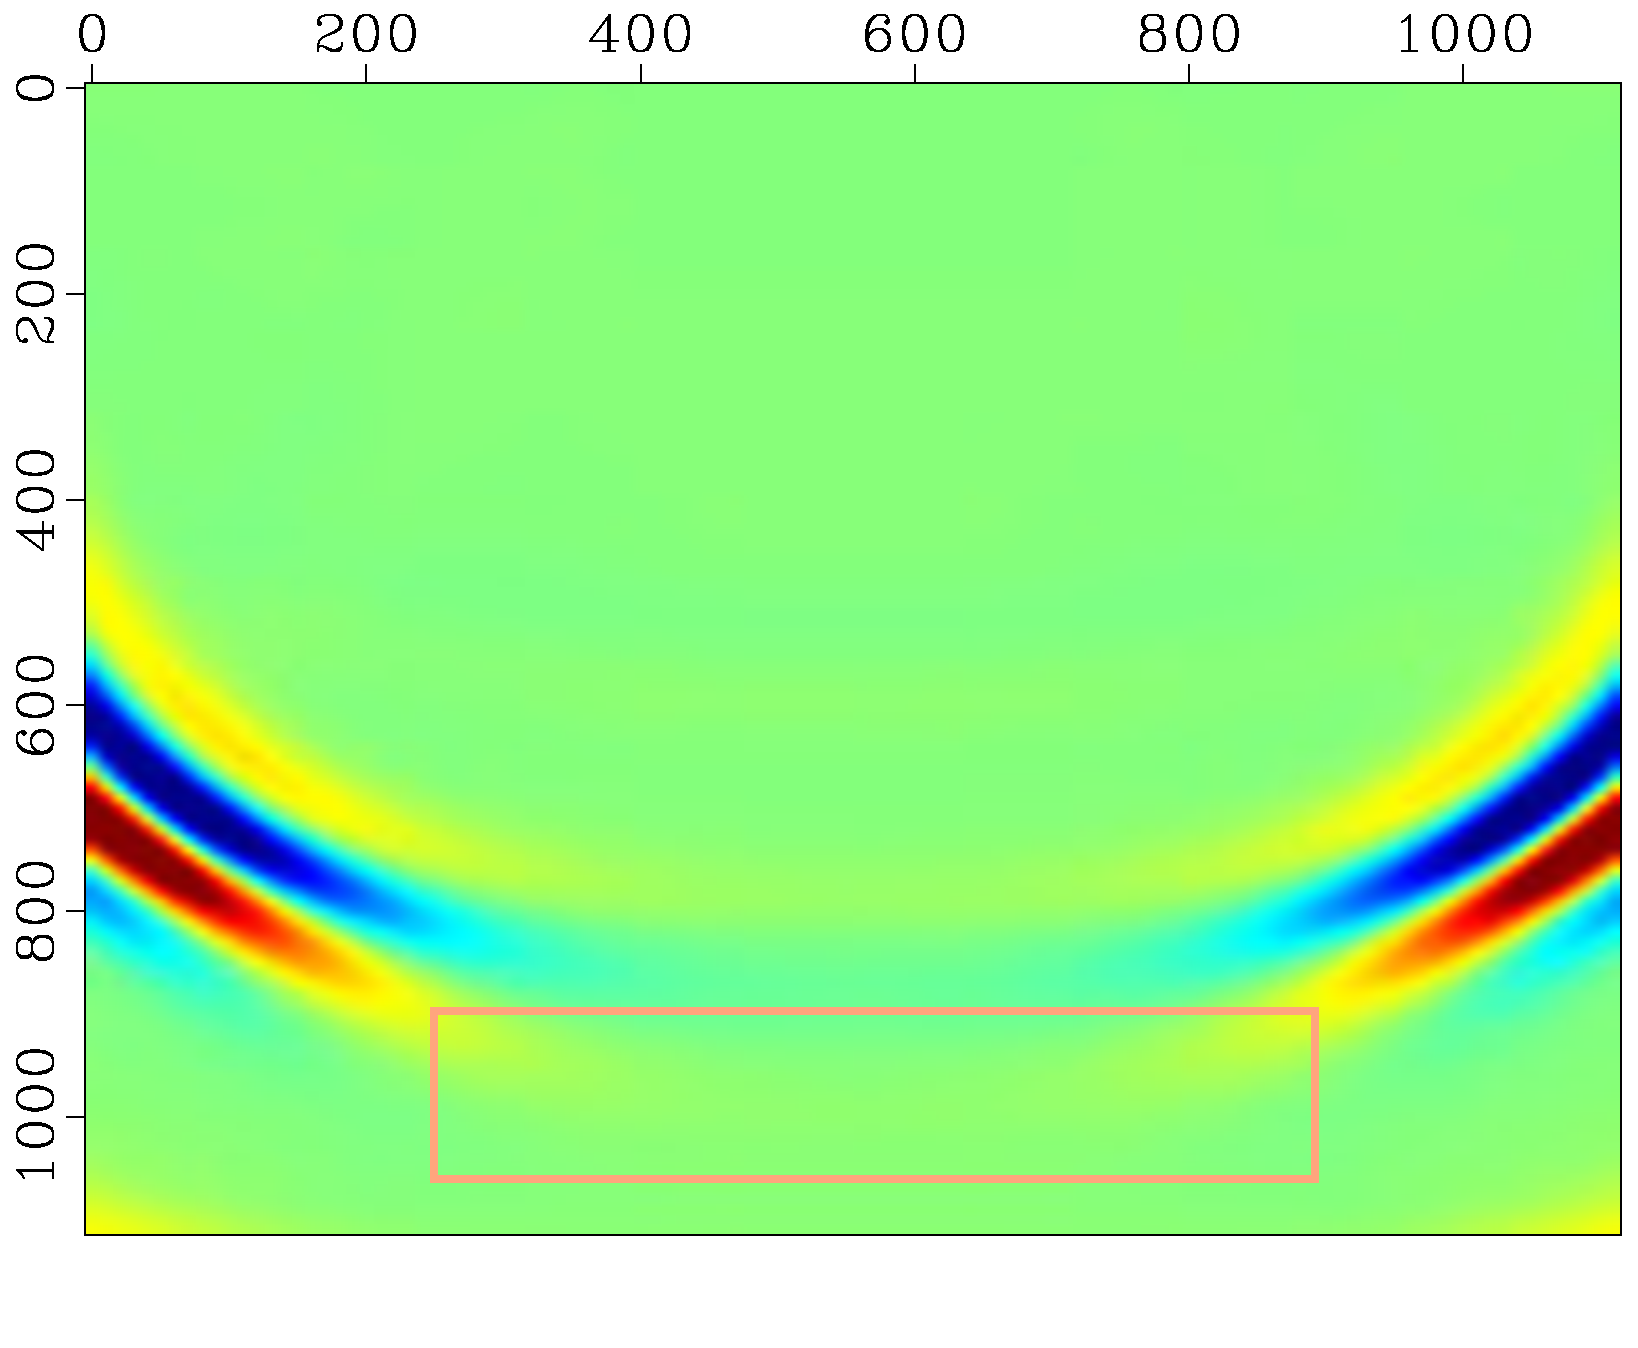
\includegraphics[height=2.2in]{q20.pdf}
        \caption{常数衰减近似的地震波正演波场在$t=0.8s$的波场快照。}
        \label{fig:常数衰减近似的地震波正演波场在$t=0.8s$的波场快照。}
    \end{subfigure}
    \caption{无衰减和常数衰减近似的地震波正演波场快照对比。}
    \label{fig:qwavefield}
\end{figure}

但在地震波波前(深度$z=900$,水平$x=500$)位置,能看到常数衰减近似算法的波前能量(图\ref{fig:无衰减的地震波正演波场在$t=0.8s$的波场快照。})比无衰减正演算法的波前能量(图\ref{fig:无衰减的地震波正演波场在$t=0.8s$的波场快照。})低。为了更直观地体现高频能量衰减,本文将两者的波场能量变换到频域,如图\ref{fig:stdqwavefield}所示。红色的曲线是标准的无能量衰减的波数与能量幅值;蓝色的曲线是常数衰减因子为$Q_s=Q_p=20$的能量图。可以看到,两条曲线的形状类似,同时在波数为6至8区间达到最大能量。但是蓝色(有衰减)曲线的最大能量却只有红色(无衰减)曲线的最大能量的一半,充分证明了能量的衰减。

\begin{figure}[ht]
\centering
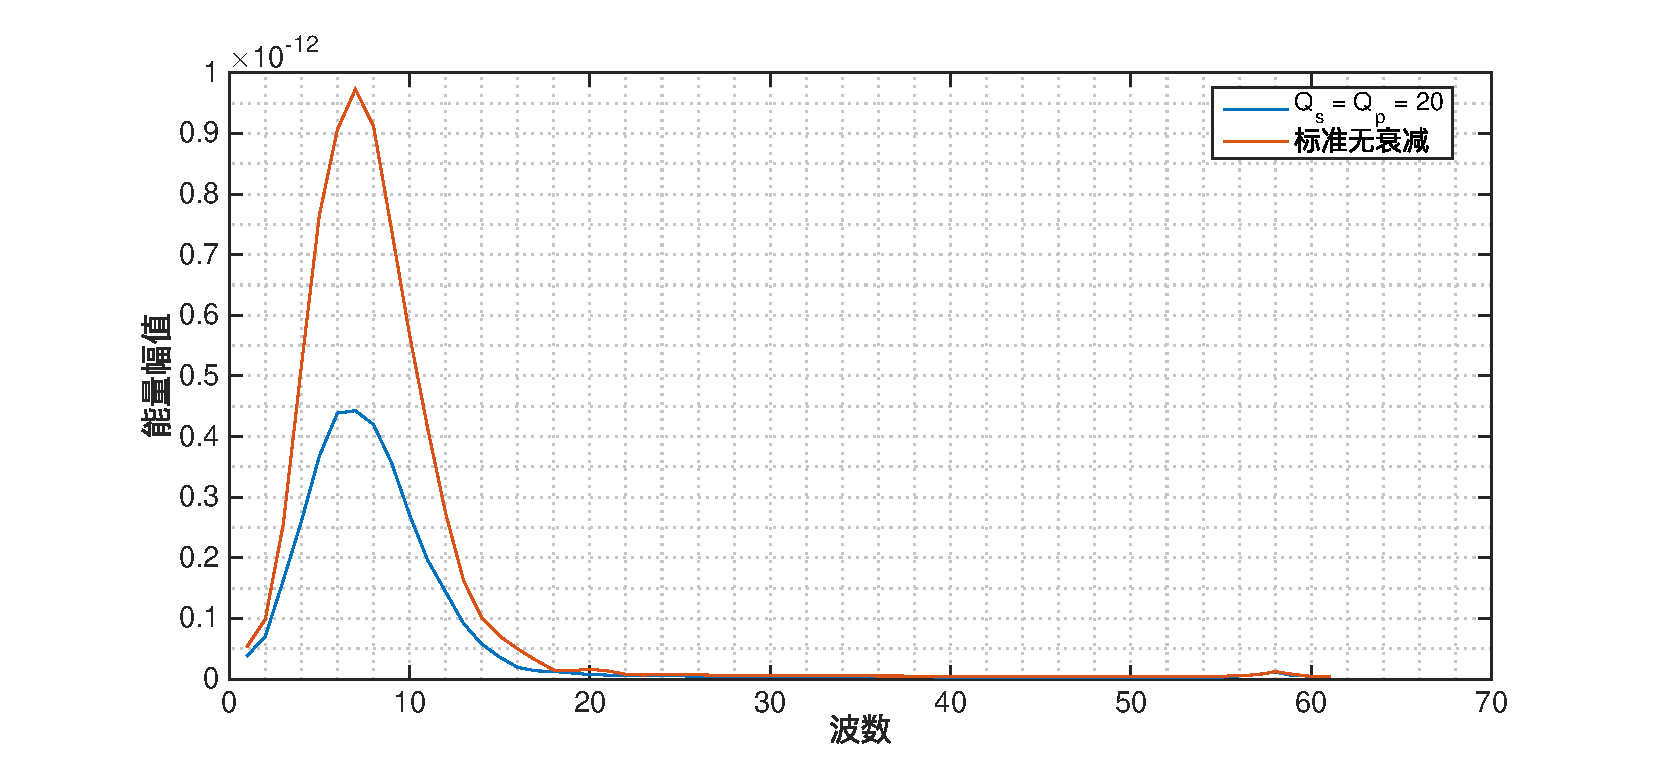
\includegraphics[width=0.9\columnwidth]{stdqwavefield.eps}
\caption{标准无衰减正演波场与常数衰减近似正演波场在$t=0.8s$处的频域能量对比。}
\label{fig:stdqwavefield}
\end{figure}

尽管图\ref{fig:无衰减的地震波正演波场在$t=0.8s$的波场快照。}和图\ref{fig:常数衰减近似的地震波正演波场在$t=0.8s$的波场快照。}能看到细微的波场差别,但这只是合成模型的正演模拟现象,地震波能量在合成模型中并不会衰减。而在真实的地震勘探中,波场能量在地球内部会不断衰减,常数衰减近似算法能够更精确地模拟真实现象。

地震波能量在不同介质中的衰减速度不同,这由衰减因子Q来描述。不同Q在地震波传播不同时间点的加速比如图\ref{fig:diffqspeedup}所示。在$t=[0s,3s]$时间内,加速比逐渐降低。这部分的加速并不是主要受益于能量衰减带来的网格空间采样变大,而是受益于地震传播初期波场更新范围的缩小。传播时间越早,需要更新的网格区域越小,因此带来的加速比越大。在$t=3s$时,地震波基本传播到整个模拟区域,因此分时动态区域算法无法带来明显的性能提升。在$t=[0,3s]$时间内,不同的衰减因子(Q)带来的加速比并不明显;但是在$t=3s$以后,传播时间越长,能量衰减的越多,根据频散和稳定性条件,空间和时间采用越大,获得的加速比也越大。当$t=8s$时,常数衰减近似正演算法取得了传统无衰减近似算法的120至190倍加速。这使得基于三维弹性波的正演、偏移和反演等算法能够在普通的集群进行数值实验模拟,极大的降低了对并行计算平台的要求。

\begin{figure}[ht]
\centering
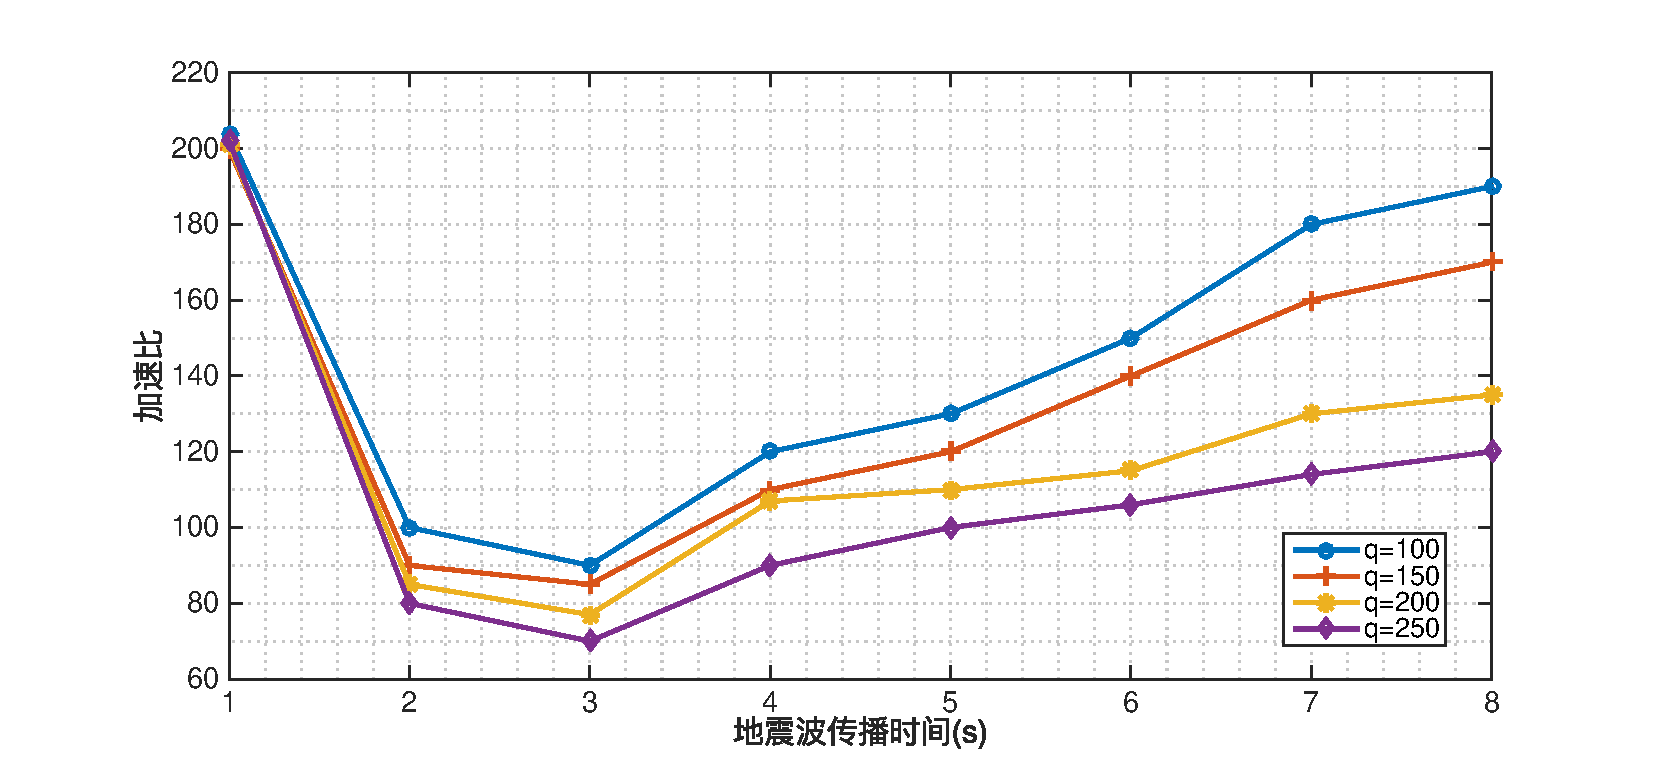
\includegraphics[width=0.9\columnwidth]{不同Q的加速比.eps}
\caption{不同Q在地震波传播不同时间点的加速比。}
\label{fig:diffqspeedup}
\end{figure}

% section 分时动态区域变分辨率正演方法 (end)

\section{集合全波形反演方法}

\subsection{设计思路}
全波形反演方法(full waveform inversion; FWI)于1984年由Tarantola提出,能准确地从人工地震记录中提取大量地下介质信息\cite{tarantola1984inversion,plessix2012full,brossier2009seismic}。该方法通过对比数值模拟合成的地震记录和实际观测的人工地震记录误差,迭代更新模型参数,从而反演地下介质模型\cite{yushu}。虽然全波形反演方法早在80年代提出,但由于该方法伴随着巨大的计算开销,直到2010年超级计算机和NVIDIA GPU,Intel MIC等加速器的兴起为全波形反演方法提供了足够的算力,该方法才逐渐成为研究热点,并为各大石油公司采用。

全波形反演方法在理论上能够很好地反演地下介质模型,但在实际生产中却面临着两大问题。一方面,全波形反演方法需要非常准确的初始速度模型作为输入,否则该算法很容易陷入局部最优\cite{virieux2009overview}。虽然地震记录中的低频信号成分能够降低对初始速度模型的要求,但是在实际生产场景中往往很难捕捉到低频信号\cite{sirgue2006importance}。另一方面全波形反演方法对地震记录数据中的噪音非常敏感,这严重影响了该算法的实际成像效果。

集合全波形反演方法(EnFWI)\cite{yushu,he2015ensemble}在传统完全反演\cite{tarantola1982generalized}(total inversion)的基础上,通过使用集合卡尔曼滤波\cite{evensen2003ensemble}中的集合协方差来近似完全反演中协方差算子,这降低了在完全反演中更新协方差算子的计算开销,使之可以在一般的分布式集群中进行计算。然而,由于速度模型中需要更新的参数数量比集合样本数量大2-4个数量级,集合卡尔曼滤波的更新增量受到很大的限制。对此,集合全波形反演方法再次引入了震源编码技术\cite{krebs2009fast}。震源编码技术将所有的震源和地震记录分别进行叠加,每次叠加时不同的震源和地震记录分别使用不同的震源编码,这克服了全波形反演算法的局部收敛\cite{castellanos2014fast}和集合卡尔曼滤波低秩空间局限性。

\subsection{算法描述}
均匀介质的声波全波形反演方法可以通过公式\ref{eq:fwi}表示:
\begin{equation}
\label{eq:fwi}
  \min_{m} \phi(m) = \sum_{i=1}^S \rho(\mbox{H}_i(m) - d_{i} ),
\end{equation}
其中$m$表示背景速度模型,$\rho(\cdot)$是一个补偿函数,$d_i=d_1, \ldots, d_S$表示观测数据(实际接收的地震记录),$\mbox{H}_i=\mbox{H}_1, \ldots, \mbox{H}_S$则表示与之相对应的第$i$个正演算子,$S$表示总勘探实验次数(每发射一炮代表一次实验)。这个优化问题通常使用如公式\ref{eq:steepest}形式的迭代算法进行求解:
\begin{equation}
\label{eq:steepest}
m_{k+1} = m_{k} + \alpha_{k}s_k,
\end{equation}
其中$s_k$表示搜索方向,$\alpha_{k}$表示步长。常用的方法包括最速下降法、共轭梯度法等等。

集合全波形反演方法在每次速度模型更新之后使用集合卡尔曼滤波对速度模型集合进一步更新,如公式\ref{eq:enkfupdate}所示:
\begin{equation}
\label{eq:enkfupdate}
\left(\mbox{H}\Psi_k^{'}(\mbox{H}(\Psi_k^{'})^T)+D_k^{'}(D_k^{'})^T\right)^{-1}\approx\left((\mbox{H}\Psi_k^{'}+D_k^{'})(\mbox{H}\Psi_k^{'}+D_k^{'})^T\right)^{-1}.
\end{equation}
其中$k$表示第$k$个迭代步,$\Psi_k=(\psi_1^k,\psi_2^k,\ldots,\psi_N^k)$表示有$N$个速度模型样本组成的背景速度场,$D=(d_1^k,d_2^k,\ldots,d_N^k)$表示添加扰动之后的观测数据集合。通过SVD分解有,
\begin{equation}
\label{eq:svd}
\mbox{H}\Psi_k^{'}+D_k^{'}=USV,
\end{equation}
其中$U$和$V$是正交矩阵,$S$是对角矩阵。结合公式\ref{eq:enkfupdate}和\ref{eq:svd},可获得集合更新方程\ref{eq:enkf2}
\begin{equation}
\label{eq:enkf2}
(\Psi_a)_k=\Psi_k+\Psi_k^{'}(\mbox{H}\Psi_k^{'})^TU(SS^T)^{-1}U^T(D_k-H\Psi_k).
\end{equation}
其中$\Psi_a$表示分析速度场。

\subsection{算法分析}
算法 \ref{alg:enfwicode} 以伪代码的形式描述了集合全波形反演算法。与传统的全波形反演不同,集合全波形反演算法首先需要初始化EnFWI分析步所需要的相关输入,如添加随机扰动后的背景速度场集合、观测数据以及EnFWI分析步所需要的参数(第\ref{ln:enfwiinit}行)。由于背景速度场集合是由同一个初始速度场添加扰动所得,剧烈的扰动会极大改变背景速度场,从而影响全波形反演的成像结果。因此,在进行正式的全波形反演迭代之前,需要执行一次EnFWI分析步计算(第\ref{ln:enfwi1enkf}行),以便为后续的迭代提供一个差异化且较为平滑的初始速度集合。

\begin{algorithm}[ht]
%\scriptsize
%\footnotesize
\small
\caption{集合全波形反演算法伪代码}\label{alg:enfwicode}
\begin{algorithmic}[1]
\State \textbf{//初始化背景速度场集合(vels)、观测数据(obsdata)、EnFWI分析步所需参数(lambdas, ratios)}
\State [vels, obsdata, lambdas, ratios] = init4enkf(); \label{ln:enfwiinit}
\State
\State \textbf{//根据初始速度场进行首次EnFWI分析步计算}
\State enkf\_analyze(vels, obsdata, lambdas, ratios); \label{ln:enfwi1enkf}
\State
\State \textbf{for} (iter = 1; iter < niter; iter++) \{ \textbf{//EnFWI收敛所需运行的总迭代次数} \label{ln:enfwiiter}
\State
\State \quad\quad \textbf{//nsamples为集合样本数目,每一个样本执行独立的震源编码FWI}
\State \quad\quad \textbf{for} (isample = 0; isample < nsamples; isamples++) \{ \label{ln:enfwisample}
\State \quad\quad\quad\quad \textbf{//生成震源编码,并对震源和观测数据进行统一编码}
\State \quad\quad\quad\quad codes = gen\_codec(nshots); \label{ln:enfwicodec}
\State \quad\quad\quad\quad [ensrc, endata, resd, prevgrad, curgrad] = init4essfwi();
\State \quad\quad\quad\quad \textbf{for} (ishot = 0; ishot < nshots; ishots++) \{
\State \quad\quad\quad\quad\quad\quad ensrc += codes[ishot] * srcs[ishot];
\State \quad\quad\quad\quad\quad\quad endata += codes[ishot] * obsdata[ishot];
\State \quad\quad\quad\quad \} \label{ln:enfwicodecend}
\State
\State \quad\quad\quad\quad \textbf{//基于震源编码的地震波正演,计算量最大的函数之一}
\State \quad\quad\quad\quad syndata = forward\_modeling(ensrc, vels[ismaple]); \label{ln:enfwiforward}
\State \quad\quad\quad\quad vsrc = endata - syndata; \label{ln:vsrc}
\State \quad\quad\quad\quad resd += cal\_residual(endata, syndata); \label{ln:resd}
\State
\State \quad\quad\quad\quad \textbf{//基于震源编码的伴随波场反传,计算量最大的函数之一}
\State \quad\quad\quad\quad [vdata, curgrad] = backward\_propagate(vsrc, vels[isamples]); \label{ln:enfwibackward}
\State \quad\quad\quad\quad updatedir = conj\_gradient(prevgrad, curgrad); \textbf{//计算更新梯度方向}
\State \quad\quad\quad\quad swap(prevgrad, curgrad);
\State
\State \quad\quad\quad\quad \textbf{//计算更新步长,计算量最大的函数之一}
\State \quad\quad\quad\quad alpha = cal\_steplen(ensrc, vels[isample], updatedir, resd);
\State \quad\quad\quad\quad update\_vel(alpha, updatedir, vels[isample]); \textbf{//根据梯度和步长更新背景速度场} \label{ln:enfwibackwardend}
\State \quad\quad \} \label{ln:enfwisampleend}
\State
\State \quad\quad \textbf{if} (iter \% enkf\_interval == 0) \{ \textbf{//每隔enkf\_interval迭代步进行EnFWI分析步计算} \label{ln:enfwienkfbegin}
\State \quad\quad\quad\quad enkf\_analyze(vels, lambdas, ratios);
\State \quad\quad \} \label{ln:enfwienkfend}
\State \} \label{ln:enfwiiterend}
\end{algorithmic}
\end{algorithm}

集合全波形反演方法与传统全波形反演的计算流程类似,都是通过迭代算法来求解(第\ref{ln:enfwiiter}到\ref{ln:enfwiiterend}行)。但由于集合全波形反演方法使用集合样本来替代传统全波形反演中的独立样本,集合全波形反演方法需要对集合中的每一个样本独立执行完成的FWI计算(第\ref{ln:enfwisample}到\ref{ln:enfwisampleend}行)。这是集合全波形反演方法引入额外计算开销的最主要原因。集合中的每一个样本都是一个独立的完整全波形反演计算,因此集合全波形反演的计算复杂度与集合的样本数量成线性相关。为了降低计算复杂度,集合全波形反演方法引入了震源编码技术,在每一个迭代步每一个样本中对所有震源和观测数据进行统一编码(第\ref{ln:enfwicodec}到\ref{ln:enfwicodecend}行),然后对编码后的震源进行线性叠加。未进行震源编码时,全波形反演需要遍历每一炮勘探实验,而进行震源编码之后,不再需要逐炮进行遍历,而是将不同位置的震源根据编码同时添加到地震波场中。震源编码技术直接将全波形反演的计算复杂度将为原来的$1/nshots$,其中$nshots$表示炮的数目。这在大规模三维石油勘探反演成像中加速效果非常明显,因为大规模石油勘探中炮击的次数通常为成千上万甚至十万个。值得注意的是,在每个迭代步每个样本的全波形反演中,所有炮击的震源和观测数据使用相同的编码,但在不同迭代步不同样本中,需要重新生成编码。

随后,以编码后的震源和当前样本速度场作为输入进行地震波正演(forward\_modeling),模拟地震波从震源发射,经过不同地下介质的传播,最后到达地震记录接收器的整个过程(时间从$t=0$到$t=nt-1$时刻,第\ref{ln:enfwiforward}行)。由于当前迭代步的速度场并不是真实的速度场,以此速度场进行正演得到的地震记录成为合成地震记录(syndata)。通过实际观测地震记录和当前合成地震记录可计算得到伴随波场震源(vsrc)和目标函数残差(resd,第\ref{ln:vsrc}行和第\ref{ln:resd}行)。全波形反演的目标则在于最小化目标函数残差,残差越小,代表当前速度模型与真实速度模型越接近。以伴随波场地震记录和当前速度模型作为输入进行地震波反传(时间从$t=nt-1$到$t=0$时刻),并与对应的正传波场进行相关(correlation)操作,可求得速度场更新的梯度和步长,用以更新当前速度模型(第\ref{ln:enfwibackward}到\ref{ln:enfwibackwardend}行)。在整个基于震源编码的全波形反演中,计算量最大的三个过程分别是地震波正传、伴随波场反传和计算更新步长。每一个过程都需要对整个波场进行从$t=0:nt-1$或$t=nt-1:0$进行更新。集合中的每一个速度场使用基于震源编码的全波形反演进行更新之后,每隔一定的迭代步执行集合卡尔曼滤波分析以进一步更新背景速度场集合(第\ref{ln:enfwienkfbegin}到\ref{ln:enfwienkfend}行),然后进入下一个迭代步继续迭代。

集合卡尔曼滤波分析步旨在利用集合替代样本,降低初始速度模型和数据噪音对算法收敛的影响,提高算法的收敛域。集合全波形反演的额外开销一方面来源于使用集合替代单独样本,在全波形反演中需要为集合中的每个样本单独更新背景速度场。在引入了震源编码之后,震源编码对所有的炮点进行叠加,极大降低了计算复杂度,减轻甚至抵消了集合样本带来的开销。

集合全波形反演另一方面的开销则是集合卡尔曼滤波分析步(简称分析步)的计算,虽然并不需要在每个迭代步中都执行分析步计算,但深入分析有利于我们更好地理解集合卡尔曼滤波分析步,并为后续的优化提供可靠的思路。

公式\ref{eq:enkf2}描述了分析速度场的更新方式。结合算法 \ref{alg:enfwicode},可发现如下计算特性:
\begin{itemize}
  \item 分析速度场的更新是所有速度模拟样本的整体更新,而不是像震源编码全波形反演中的每个速度模型独立更新。
  \item 分析速度场更新的主要计算是大型矩阵和向量代数运算,包括矩阵加法、乘法、转置、求逆等计算密集型的操作,这与太湖之光强大的计算能力十分吻合。
  \item 正演算子$\mbox{H}$,即算法 \ref{alg:enfwicode} 中的forward\_modeling函数仍旧在公式中扮演者重要的作用。通过程序用时解剖(profile)发现,正演算子$\mbox{H}$依旧是EnFWI分析步最耗时的函数,但与算法 \ref{alg:enfwicode}不同,分析步中的正演算子无需设计IO存储,因为分析步中不需要进行地震波反传操作并进行相关(correlation)操作。
\end{itemize}

\begin{table}[ht]
\centering
\caption{集合卡尔曼滤波分析步中不同计算操作耗时百分比。}
\label{tb:enkfprofile}
\begin{tabular}{ccccccc}
\hline
计算操作  & 矩阵加法  & 矩阵乘法  & 矩阵求逆   & 矩阵转置  & 正演算子   & 其他    \\\hline
所占百分比 & 3.2\% & 8.5\% & 17.0\% & 4.3\% & 58.9\% & 8.1\% \\\hline
\end{tabular}
\end{table}
表\ref{tb:enkfprofile}总结了集合卡尔曼滤波分析步中不同计算操作耗时百分比。可以发现,优化分析步计算的核心是优化正演算子和矩阵求逆运算。其中正演算子占了近60\%的总计算开销,因此前文提出的分时动态变分辨率正演方法也可用于优化集合全波形反演中的正演算子。


% section 实验结果与分析 (end)

\section{本章小结} % (fold)
正演的本质是仿真地震物理过程,这是地震模拟的核心,同时也是反演的基础。正演算法的性能也直接决定着反演的性能。本研究讨论基于波动方程的正演和全波形反演算法,从算法层面提出优化性能的两种方法——分时动态变分辨率正演方法和集合全波形反演方法。

分时动态区域正演算法利用地震波传播初期未填充模拟区域的现象,通过分时确定最大传播范围,忽略波前未到达的区域,从而提升计算效率。分时变分辨率正演方法利用地震波能量在地球内部不断衰减的特性,结合稳定性和频散条件,分时动态改变波场时空分辨率,并从二维声波方程扩展到三维弹性波方程。随后本章将分时动态区域正演和分时变分辨率正演方法结合使用,提出分时动态变分辨率正演方法作为本研究基础正演方法,并验证了分时动态变分辨率正演方法能够保证正演精度的同时获得了可观的性能提升。

最后本章在全波形反演方法的基础上提出基于震源编码的集合全波形反演方法。集合全波形反演方法通过集合卡尔曼滤波的集合协方差来近似完全反演中协方差算子,然后引入了震源编码技术将所有的震源和地震记录分别进行叠加,在扩大全波形反演收敛域和降低噪音敏感度的同时极大了提升了计算效率。
